\documentclass[12pt,a4paper]{report}

% Packages (template preamble kept; changes against the template are marked FIX)
% FIX: Times under pdfLaTeX (template, Overleaf); TeX Gyre Termes, the same metrics, when a local
% build uses XeTeX (Tectonic), where the times package has no effect.
\usepackage{iftex}
\ifXeTeX
  \usepackage{fontspec}
  \setmainfont{texgyretermes}[Extension=.otf,UprightFont=*-regular,BoldFont=*-bold,ItalicFont=*-italic,BoldItalicFont=*-bolditalic]
  \setmonofont{texgyrecursor}[Extension=.otf,UprightFont=*-regular,BoldFont=*-bold,ItalicFont=*-italic,BoldItalicFont=*-bolditalic]
\else
  \usepackage{times}            % Times New Roman font
\fi
\usepackage{setspace}           % Line spacing
\usepackage[a4paper, left=1.5in, right=1in, top=1in, bottom=1in]{geometry}
\usepackage{titlesec}           % Chapter/section formatting
\usepackage{fancyhdr}           % Header/Footer
\usepackage{graphicx}           % Figures
\usepackage{tocloft}            % TOC formatting
\usepackage{etoolbox}           % needed for patching TOC entries
% FIX: lipsum, xcolor and the second titlesec line of the template are removed (unused).
% FIX: packages the chapters need are added.
\usepackage{amsmath}            % Equations
\usepackage{amssymb}            % Symbols
\usepackage{float}              % [H] placement
\usepackage{array}              % Table column types
\usepackage{tabularx}           % Tables that fit the text width
\usepackage{longtable}          % Tables that break across pages
\usepackage{multirow}           % Merged table cells
\usepackage{url}                % URLs in references
\usepackage{enumitem}           % List spacing
\usepackage{caption}            % Captions
\usepackage[hidelinks]{hyperref} % FIX: hidelinks removes the coloured link boxes

% Left-aligned fixed-width column, used by the tables in the chapters
\newcolumntype{L}[1]{>{\raggedright\arraybackslash}p{#1}}

% FIX: figures are looked up in figures/ (the logos stay in the report root)
\graphicspath{{figures/}}

% Line spacing
\onehalfspacing
\setlength{\emergencystretch}{2em} % FIX: avoids text running into the margin
% FIX: float placement that fills pages instead of leaving gaps before tables and figures
\renewcommand{\topfraction}{0.85}
\renewcommand{\bottomfraction}{0.7}
\renewcommand{\textfraction}{0.12}
\renewcommand{\floatpagefraction}{0.75}
\setcounter{topnumber}{3}
\setcounter{bottomnumber}{2}
\setcounter{totalnumber}{4}


% Title formatting
\titleformat{\chapter}[hang]{\bfseries\centering\LARGE}{Chapter \thechapter}{1em}{}
\titleformat{\section}[hang]{\bfseries\Large}{\thesection}{1em}{}

% Fancy Header/Footer
\setlength{\headheight}{15pt}   % FIX: fancyhdr needs at least 14.5pt for a 12pt header
\pagestyle{fancy}
\fancyhf{}
% FIX: the header carries the official project title
\lhead{\textit{AI Powered Pothole Detection and Intelligent Route Optimization System}}
\lfoot{\textit{Dept. of CSE,BMSCE}}
\rfoot{\textit{Page \thepage}}

% Make chapter pages use fancy style
\makeatletter
\let\ps@plain\ps@fancy
\makeatother

\begin{document}

% ---------- FRONT MATTER: ROMAN NUMBERS ----------
\pagenumbering{roman}
\setcounter{page}{1}

% ----- Title Page -----
% FIX: the template's "Group Number" line (with its stray backslash) is removed; identity details
% are copied from the Phase 1 report.
\begin{titlepage}
  \thispagestyle{empty}
  \centering

  {\Huge \textbf{AI Powered Pothole Detection and Intelligent Route Optimization System}}\\[1.0cm]
  
\includegraphics[width=0.18\linewidth]{VTU-Logojpg.jpg}\\[0.9cm]
  {\Large \textbf{PROJECT REPORT}}\\[0.2cm]
  {\large \textit{Submitted by}}\\[0.5cm]
  {\large Zain Mahedi (1WA23CS056)}\\
  {\large Thanu George (1WA23CS019)}\\
  {\large Vikas Shashi (1WA23CS043)}\\
  {\large Tanish Agrawal (1WA23CS008)}\\[0.7cm]
  {\itshape in partial fulfillment for the award of the degree of}\\[0.15cm]
  {\Large \textbf{BACHELOR OF ENGINEERING}}\\[0.2cm]
  {\large in}\\[0.2cm]
  {\Large \textbf{COMPUTER SCIENCE AND ENGINEERING}}\\[0.9cm]
  {\large Under the Guidance of}\\
  {\large \textbf{Dr. Seema Patil}}\\
  {\large Associate Professor, Department of CSE, BMSCE}
  \vfill
  
\includegraphics[width=0.18\linewidth]{bmscelogo.jpg}\\[0.5cm]
  {\Large \textbf{B.M.S. COLLEGE OF ENGINEERING}}\\
  {\large (Autonomous Institution under VTU)}\\
  {\large BENGALURU - 560019}\\
  {\large Academic Year - 2026--2027}

\end{titlepage}
% ----- Certificate -----
\chapter*{Certificate}
\thispagestyle{empty}
\vspace{2cm}
This is to certify that the project report entitled \textbf{``AI Powered Pothole Detection and Intelligent Route Optimization System''} is a bonafide work carried out by \textbf{Zain Mahedi (1WA23CS056)}, \textbf{Thanu George (1WA23CS019)}, \textbf{Vikas Shashi (1WA23CS043)} and \textbf{Tanish Agrawal (1WA23CS008)} in partial fulfillment of the requirements for the award of the degree of \textbf{Bachelor of Engineering} in \textbf{Computer Science and Engineering}, under my supervision during the academic year 2026--2027.

\vspace{2cm}
\begin{flushleft}
Guide Signature\hspace{30mm} HoD signature \hspace{25mm} Principal Signature\\
(Dr. Seema Patil) \hspace{25mm} Dr. Kavitha Sooda \hspace{19mm} Dr. Bheemsha Arya
\end{flushleft}
\vspace{2cm}
\begin{flushleft}
Name and signature of Examiners along with date \\
\vspace {1cm}
Examiner 1 \\
\vspace {1cm}
Examiner 2 \\

\end{flushleft}



% ----- Abstract -----
% The body text is in chapters/abstract.tex (heading and page style are set here).
\chapter*{Abstract}
\thispagestyle{empty}
Potholes cause accidents and damage vehicles, yet municipal bodies still find most of them through complaints and manual surveys, and navigation applications choose routes with no information about the road surface. This project rebuilds an earlier segmentation-based prototype as a system that detects potholes in forward-facing road video, places them on a map and compares routes by the potholes expected along them.

Detection is single-class box detection with YOLOv8s. We prepared RDD2022 and HRP4K as one pothole class, grouped near-duplicate images by perceptual hash so that no validation or test image has a training image within 8 bits, and kept 203 images from a third dataset that labels manholes for evaluation only. Thresholds were chosen on validation data, and confidence intervals come from a group bootstrap.

The deployed baseline, trained on RDD2022 at 640 px, reached mAP\textsubscript{50} 0.497 [0.443, 0.555] on the held-out RDD2022 test split. An experimental candidate fine-tuned on RDD2022 and HRP4K at 1280 px raised mAP\textsubscript{50} on the HRP4K test split from 0.018 to 0.454, a gain that comes from training on that data. On RDD2022 its mAP\textsubscript{50} was 0.0445 lower (paired interval [$-$0.0864, $-$0.0059]), and it did not demonstrate fewer false positives or less confusion with manholes, so the baseline remains deployed. Our own recordings have no labels and were compared only qualitatively.

The system covers video and GPS ingestion, a motion-aware tracker, merging of sightings into mapped potholes, snapping to an OpenStreetMap road graph, a Dijkstra route planner whose cost adds expected potholes to distance, a FastAPI backend with SQLite storage and a five-tab browser interface. All 1,101 automated tests pass; the interface has no behaviour tests. For each road segment the system records a pothole count, surveyed length and rate per 100 m, but no severity or condition grade. Route comparison is demonstrated on a synthetic session, because our recordings cover only about 1,020 m of road.

%-------------Declaration ----------
\chapter*{DECLARATION}
\thispagestyle{empty}
We, hereby declare that the Major Project Phase-2 work entitled ``AI Powered Pothole Detection and Intelligent Route Optimization System'' is a bonafide work and has been carried out  by us under the guidance of Dr. Seema Patil, Associate Professor, Department of Computer Science and Engineering, B.M.S. College of Engineering, Bengaluru, in partial  fulfillment of the requirements of the degree of Bachelor of Engineering in Computer Science  and Engineering of Visvesvaraya Technological University, Belagavi.
I further declare that, to the best of my knowledge and belief, this project has not been  submitted either in part or in full to any other university for the award of any degree.
\vspace{0.3cm}
\begin{flushleft}
Candidate details:
\end{flushleft}
\vspace{0.1cm}
\begin{center}
\begin{tabular}{|c|l|c|c|}
\hline
\textbf{SL. NO.} & \textbf{Student Name} & \textbf{USN} & \textbf{Student's Signature} \\
\hline
1 & Zain Mahedi & 1WA23CS056 & \\
\hline
2 & Thanu George & 1WA23CS019 & \\
\hline
3 & Vikas Shashi & 1WA23CS043 & \\
\hline
4 & Tanish Agrawal & 1WA23CS008 & \\
\hline
\end{tabular}
\end{center}
\begin{flushleft}
Place: Bengaluru \\
Date: \\
\end{flushleft}
Certified that these candidates are students of Computer Science and Engineering Department  of B.M.S. College of Engineering. They have carried out the project work of titled ``AI Powered Pothole Detection and Intelligent Route Optimization System'' as Major Project Phase-2  work. It is in partial fulfillment for completing the requirement for the award of B.E. degree  by VTU. The works is original and duly certify the same.
\vspace{1cm}
\begin{flushleft}
Guide Name: Dr. Seema Patil \\
Date: \\
Signature \\
\end{flushleft}
% ----- Acknowledgment -----
\chapter*{Acknowledgment}
\thispagestyle{empty}
We are thankful to our guide, \textbf{Dr. Seema Patil}, Associate Professor, Department of Computer Science and Engineering, B.M.S. College of Engineering, who advised and encouraged us at every stage of this project.

We thank \textbf{Dr. Kavitha Sooda}, Head of the Department of Computer Science and Engineering, for giving us the facilities and support this work required, and \textbf{Dr. Bheemsha Arya}, Principal, B.M.S. College of Engineering, for allowing us to take up this project.

The project coordinators, faculty and non-teaching staff of the department helped us throughout, and we thank them. We also thank the creators of the open-source tools and public datasets used in this work, including Ultralytics YOLOv8, PyTorch, OpenStreetMap and OSRM.

Our families and friends supported us the whole way, and we thank them too.
\newpage
% ----- TOC, LoF, LoT -----
\tableofcontents
\thispagestyle{empty}
\newpage
\listoffigures
\thispagestyle{empty}
\newpage
\listoftables
\thispagestyle{empty}

% ---------- MAIN MATTER: ARABIC NUMBERS ----------
\clearpage
\pagenumbering{arabic}
\setcounter{page}{1}

% ----- Chapters -----
% FIX: no section numbers are typed into the chapter files (the template's "1.1 1.1" defect).
\chapter{Introduction}\label{ch:intro}

\section{Overview}
Potholes form when water seeps into cracked asphalt and traffic breaks the weakened surface apart. On Indian roads they slow journeys, damage vehicles and cause accidents. This report describes the second phase of our project on pothole detection and pothole-aware route recommendation. In the first phase (Phase 1) we built a prototype around a YOLOv8s-seg segmentation model, ByteTrack tracking, a rule-based severity rating, an Android recorder and a route planner that queried a public OSRM server. Its evaluation could not tell us whether it would work on footage unlike its training data, so in this phase we rebuilt the system from the beginning. The rebuilt software, internally named RoadSense and called \emph{the system} in this report, takes a forward-facing road video and a GPS log, detects potholes, places each pothole once on a road map, records how much road each recording actually covered, and uses this to compare routes between two points.

\subsection{Problem Statement}
Municipal bodies still learn about most potholes from citizen complaints and occasional manual surveys, which are slow and rarely give an exact location. Navigation applications, as far as we know, choose routes by distance and traffic and say nothing about the road surface. Camera-based detection can fill this gap, but a detector is only useful if it has been evaluated on data that differs from its training data. Phase 1 reported high scores on a test split drawn from the same recordings as its training data and performed poorly on forward-facing footage that we recorded ourselves.

The problem therefore has four parts: (i) detect potholes in forward-facing video with a detector whose data splits and evaluation are controlled for leakage and report their uncertainty; (ii) turn detections into a map on which each physical pothole appears once, on a named road segment; (iii) record which road has actually been surveyed, so that an unrecorded road is not mistaken for a clean one; and (iv) recommend routes that trade distance against expected potholes and state how much evidence supports each recommendation.

\section{Motivation}
The Ministry of Road Transport and Highways (MoRTH) reports 3,625 pothole-related accidents in 2021 and 4,446 in 2022, with 1,481 and 1,856 persons killed \cite{morth2023road}. Potholes are one contributing factor among several, and we do not claim that they dominate road safety. Two-wheeler riders are the most exposed, and our own recordings in Bengaluru were made from such a vehicle.

A manual road survey needs trained staff and special equipment, which is why most roads are inspected only once in a while. A phone or dashcam, on the other hand, records the road on every trip, and a real-time detector of the YOLO family \cite{redmon2016yolo,jocher2023yolov8} can check that footage for potholes on ordinary hardware. Our deployed model takes 8.16 ms per frame on average at $640 \times 640$ on a laptop GPU (Chapter~\ref{ch:requirements}). What took far more effort was knowing whether the detector could be trusted on footage it had never seen, because a model that scores well on one dataset often scores much lower on another \cite{torralba2011unbiased,koh2021wilds}. We ran into exactly this in Phase 1, and it is the main reason we rebuilt the evaluation before adding anything to the application.

\section{Objective}
We set seven objectives for this phase. Chapter~\ref{ch:results} comes back to each of them and reports how far it was achieved.
\begin{enumerate}[itemsep=0pt]
  \item \label{obj:data} Build training and evaluation sets that cannot leak into each other. RDD2022 and HRP4K are reduced to a single pothole class, near-duplicate images are grouped by perceptual hash so that each group stays within one split, and every excluded image is logged.
  \item \label{obj:baseline} Train a YOLOv8s baseline on RDD2022 at 640 px that can be reproduced exactly, using a fixed seed, a saved configuration and a checkpoint identified by its hash.
  \item \label{obj:protocol} Evaluate the models in a way that shows how certain each result is. Thresholds are picked on validation data alone, results carry group-bootstrap 95\% confidence intervals, models are compared in pairs, and an external set containing manholes is kept purely for testing.
  \item \label{obj:finetune} Fine-tune the baseline at 1280 px on RDD2022 together with HRP4K, and check whether the resulting candidate does better than the baseline on held-out test data.
  \item \label{obj:pipeline} Connect detection to the map. Potholes are detected and tracked, each is given a GPS position, repeated sightings of the same pothole are merged, and the result is attached to the road network along with how much of each road was actually surveyed.
  \item \label{obj:routing} Implement pothole-aware routing on an OpenStreetMap graph with a cost that adds an expected-pothole penalty to distance, reporting how much of each route was surveyed.
  \item \label{obj:backend} Provide a tested backend (HTTP API, background jobs, database, command line) and a web interface for upload, inspection and route planning.
\end{enumerate}

\section{Scope}
The work covers single-class pothole detection with bounding boxes in forward-facing RGB video, the data preparation and evaluation above, geotagging from a GPS log, mapping onto an OpenStreetMap road network, route comparison, and a web interface served by the same process as the API, for a single local user.

Several things are outside the scope or only partly done. The system does not estimate pothole size or severity and produces no road condition score or grade. For each road segment it stores the number of mapped potholes, the surveyed length and the rate per 100 m, and for each route an evidence level. There is no authentication, no database migration and no Android recorder. The web interface has no automated tests. Our own recordings have no ground truth, so no accuracy figure exists for them, and they cover only about 1,020 m of road in seven disconnected stretches, so route comparison is demonstrated on a synthetic session. The 1280 px candidate model is experimental and is not deployed.

\section{SDG Justification}
For SDG 9 (Industry, Innovation and Infrastructure, Target 9.1), an ordinary video and GPS log become mapped potholes on road segments that carry their surveyed length, so a road authority can see which roads were recorded and what was found without a survey vehicle. The output is a count and a rate, not a pavement condition index such as ASTM D6433 \cite{astm2020d6433}, so it can direct inspections but does not replace them.

For SDG 11 (Sustainable Cities and Communities, Target 11.2), the route planner offers up to three routes, from the shortest to the strongest pothole avoidance, with the potholes passed and the surveyed share of each. It has been demonstrated on a synthetic session only.

SDG 3 (Good Health and Well-being, Target 3.6) concerns road injuries, and potholes are a recorded cause of road accidents \cite{morth2023road}. A camera records a pothole before a vehicle hits it, unlike accelerometer methods \cite{eriksson2008pothole}. We have measured no effect on accidents and make no safety claim beyond providing the information.

\subsection{How the SDGs are addressed in the implementation}
Table~\ref{tab:ch1-sdg} links each goal to the parts of the implemented system that serve it, the place in this report where each part is designed, built and tested, and what the evidence does and does not show.

\begin{table}[!htbp]
\centering
\small
\renewcommand{\arraystretch}{1.2}
\begin{tabular}{|L{2.0cm}|L{4.9cm}|L{2.3cm}|L{3.6cm}|}
\hline
\textbf{SDG and target} & \textbf{Implemented components} & \textbf{Where in this report} & \textbf{Evidence and limits} \\
\hline
SDG 9, Target 9.1 (resilient infrastructure) & Video and GPS ingestion, YOLOv8s detector, motion-aware tracker and geotagging turn ordinary phone or dashcam footage into sightings; the map builder merges them into mapped potholes, snaps them to OpenStreetMap road segments and stores per segment the pothole count, surveyed length and rate per 100 m; the API and map layers show recorded potholes and surveyed road & Sections~\ref{sec:ch4-pipeline}, \ref{sec:ch4-db}, \ref{sec:ch5-modules}; tests in Section~\ref{sec:ch6-tests} & Detector mAP\textsubscript{50} 0.497 on held-out RDD2022 test data; map-building and API tests pass. Counts and rates only, not a condition index; no labelled data from our own roads \\
\hline
SDG 11, Target 11.2 (safe, sustainable transport) & Route planner on a local OpenStreetMap graph with a cost that adds expected potholes to distance and treats unsurveyed road as unknown; up to three routes with distance, potholes passed, surveyed share and evidence level; route-planner tab in the web interface & Sections~\ref{sec:ch4-route}, \ref{sec:ch5-modules}; tests in Section~\ref{sec:ch6-tests} & Routing tests pass; route comparison demonstrated on a synthetic session, because our recordings cover only about 1,020 m \\
\hline
SDG 3, Target 3.6 (fewer road injuries) & Forward-facing camera detection that records a pothole before a vehicle reaches it; avoidance setting in the route planner; route caveats that never call a road safe or pothole-free & Sections~\ref{sec:ch4-pipeline}, \ref{sec:ch4-route}; results in Section~\ref{sec:ch6-results} & Information support only; the detector has known false positives on covers and patches, and no effect on accidents was measured \\
\hline
\end{tabular}
\caption{How each Sustainable Development Goal is addressed in the implemented system.}
\label{tab:ch1-sdg}
\end{table}

\section{Existing System}
Pothole information in Indian cities comes mainly from complaints, social media and periodic inspection. Survey vehicles with laser, depth or LiDAR sensors measure the surface accurately \cite{ma2022review,kang2017pothole} but cover little of the network. Automatic methods are vibration-based, vision-based or based on three-dimensional reconstruction \cite{kim2022review,ma2022review}. Most vision work since the road-damage datasets of Maeda et al. and Arya et al. \cite{maeda2018road,arya2022rdd2022} stops at the detector; the few systems that add mapping or routing are preprints without independent evaluation \cite{sahoo2025iwatchroadv2,balakuntala2013pothole}.

\subsection{The earlier implementation (Phase 1)}
Phase 1 trained a YOLOv8s-seg model \cite{jocher2023yolov8} at 640 px on every fifth frame of paired road and mask videos (3,720 training, 1,240 validation and 1,230 test frames from 372, 124 and 123 videos). It tracked detections with ByteTrack \cite{zhang2022bytetrack}, rated each pothole Mild, Moderate or Severe from the area, edge irregularity and elongation of its mask, interpolated positions from an optional GPS log, and counted Severe and Moderate potholes within 20 m of the alternatives returned by a public OSRM server \cite{luxen2011osrm}. An Android application recorded video and GPS. The Phase 1 report gives a mask precision of 0.959, recall of 0.907 and mAP\textsubscript{50} of 0.905 on its own in-distribution test split.

Four limitations motivated the rebuild. First, the severity thresholds were calibrated on a small sample, not on human grades, and the pixel area of a pothole depends on camera distance (Phase 1 README). Second, the only evaluation was on a split from the same videos and camera set-up as training, which says nothing about other cameras or viewpoints. Third, the Phase 1 report records that a forward-facing recording made on a two-wheeler was over-segmented. Fourth, routing counted potholes near each route, so an unrecorded road and a recorded clean road looked the same, and it depended on an external server. Chapter~\ref{ch:results} compares the Phase 1 model qualitatively with the new models on our own recordings.

\section{Proposed System}
Table~\ref{tab:ch1-comparison} summarises how the rebuild differs. Following the design decisions taken at the start of this phase, it uses forward-facing footage only, single-class box detection without segmentation or severity, RDD2022 as the first training set with our own footage reserved for testing, and no Android application.

\begin{table}[!htbp]
\centering
\small
\renewcommand{\arraystretch}{1.2}
\begin{tabular}{|L{2.4cm}|L{5.0cm}|L{5.6cm}|}
\hline
\textbf{Aspect} & \textbf{Phase 1 system} & \textbf{Rebuilt system} \\
\hline
Task & Instance segmentation with a Mild, Moderate or Severe rating & Single-class box detection; no severity \\
\hline
Training data & Paired road and mask videos, every fifth frame & RDD2022 (HRP4K added for the candidate); near-duplicates grouped by perceptual hash \\
\hline
Evaluation & In-distribution test split & Held-out splits, external manhole probe, group-bootstrap 95\% intervals \\
\hline
Tracking & ByteTrack on every fifth frame & Own motion-aware IoU tracker; stride chosen from GPS speed \\
\hline
Mapping & Positions on a map & Merge sightings within 8 m, snap to the nearest road edge within 30 m, record surveyed length \\
\hline
Routing & Public OSRM alternatives, potholes within 20 m & Dijkstra on a local OpenStreetMap graph; cost adds expected potholes to length \\
\hline
Recording & Android application & Video and GPS CSV file uploaded \\
\hline
\end{tabular}
\caption{Differences between the Phase 1 system and the rebuilt system.}
\label{tab:ch1-comparison}
\end{table}

The deployed detector is the \emph{baseline}, a YOLOv8s model trained on RDD2022 at 640 px. The \emph{candidate}, fine-tuned from it on RDD2022 and HRP4K \cite{chen2026hrp4k} at 1280 px, is an experiment and is not deployed, because it showed no reduction in false positives or manhole confusion and lost some accuracy on RDD2022 (Chapter~\ref{ch:results}). Around the detector, the application processes uploads as background jobs, stores confirmed detections as sightings, rebuilds the pothole map after each job, and plans up to three routes with their potholes passed, surveyed share and evidence level. Chapters~\ref{ch:requirements} to~\ref{ch:implementation} give the requirements, design and implementation.

\section{Work Plan}
Table~\ref{tab:ch1-workplan} lists the phases of the work.

\begin{table}[!htbp]
\centering
\small
\renewcommand{\arraystretch}{1.2}
\begin{tabular}{|c|L{8.6cm}|L{3.6cm}|}
\hline
\textbf{Phase} & \textbf{Work} & \textbf{Period} \\
\hline
1 & Literature survey, problem definition and the Phase 1 prototype and report & Phase-1 (previous semester) \\
\hline
2 & Design decisions for the rebuild; RDD2022 conversion to one pothole class, near-duplicate grouping and leakage-controlled splits & August 2026 \\
\hline
3 & Baseline YOLOv8s training on a rented GPU; evaluation protocol with validation-only thresholds and group-bootstrap intervals & August -- September 2026 \\
\hline
4 & Detection pipeline: motion-aware tracking, GPS geotagging, merging of sightings and road snapping & September 2026 \\
\hline
5 & Road graph and route planner, FastAPI backend, SQLite database and web interface & September -- October 2026 \\
\hline
6 & Own road recordings; HRP4K and manhole-probe review; candidate fine-tuning at 1280 px & October 2026 \\
\hline
7 & Automated testing, evaluation and comparison on own recordings, report and presentation & October 2026 \\
\hline
\end{tabular}
\caption{Work plan.}
\label{tab:ch1-workplan}
\end{table}

\chapter{Literature Survey}\label{ch:literature}

\section{Overview}
We review the literature by theme: sensing approaches, learned detectors, road-damage datasets, methodological issues that affect how far published scores can be trusted, and systems that link detection to maps and routes. For each theme we note what it means for this project. Results are given as the cited authors report them; results of this project are in Chapter~\ref{ch:results}.

\section{Detailed Survey}

\subsection{Sensor-based and three-dimensional approaches}
Recent surveys group pothole detection into vibration-based, vision-based and three-dimensional reconstruction-based methods \cite{kim2022review,ma2022review,safyari2024review}. Vibration methods infer a pothole from the shock a vehicle receives. Eriksson et al. equipped seven taxis in Boston with accelerometers and GPS and report a false-positive rate below 0.2\% on good road segments \cite{eriksson2008pothole}; Mednis et al. run similar detectors on Android phones and report true positive rates up to 90\% \cite{mednis2011real}. These methods need no camera, but a pothole is recorded only after a vehicle has hit it.

Three-dimensional methods measure the surface directly. Fan et al. fit a quadratic road surface to stereo disparity and flag deviating points, reporting about 98.7\% accuracy on their own data \cite{fan2020pothole}; Kang and Choi combine a 2-D LiDAR with a camera \cite{kang2017pothole}; Dhiman and Klette compare stereo-vision and deep-learning techniques \cite{dhiman2020pothole}. Depth gives a physical measure that one image cannot, at the cost of extra hardware, and each study reports figures on its own data. We chose a single forward-facing camera and a GPS log, both of which any phone already has. Without depth information the system cannot measure how large or deep a pothole is, so it does not estimate size or severity.

\subsection{Learned object detectors}
Faster R-CNN is the usual example of a two-stage detector. It first proposes candidate regions and then classifies each of them \cite{ren2017faster}, which tends to be accurate but slower than a single-stage design. YOLO drops the proposal step and predicts boxes and class scores for the whole image in one pass; its authors report 45 frames per second for the base model \cite{redmon2016yolo}. This single-pass design is what lets us process road video on a laptop GPU.

We use Ultralytics YOLOv8. It was released as software without a paper, so we cite it in the form its documentation gives \cite{jocher2023yolov8}. We use the YOLOv8s size without architectural changes. Recent work modifies YOLOv8 for road damage: Zeng and Zhong report a lightweight YOLOv8n variant on RDD2022 with a gain of 1.4 mAP points over their baseline \cite{zeng2024yolov8pd}. Such papers report single-split point estimates, so a reader cannot tell whether the gains exceed the variation between splits or runs. Keeping the architecture fixed lets us study the effect of data and evaluation choices on their own.

\subsection{Road-damage datasets and challenges}
Maeda et al. released 9,053 smartphone images with 15,435 damage instances in eight classes \cite{maeda2018road}. RDD2020 grew this to 26,336 images from India, Japan and the Czech Republic \cite{arya2021rdd2020}; the 2020 challenge on it was won by a YOLO-based ensemble with F1 scores of 0.67 and 0.66 on two test sets \cite{arya2020grddc}. Arya et al. also studied models trained on one country and applied to others \cite{arya2021multicountry}. RDD2022 contains 47,420 images from six countries with four damage types: longitudinal, transverse and alligator cracks, and potholes \cite{arya2022rdd2022}. Its 2022 challenge reported per-country leaderboards and a best F1 of 76\% from an ensemble of YOLO and Faster R-CNN models \cite{arya2022crddc}. For our purposes RDD2022 has two limitations: the pothole is one of four classes, so a single-class detector requires relabelling, and most of its images are small, between 600 and 720 px square.

HRP4K approaches the problem from the other side. Chen et al. provide 6,003 forward-view images at $3840 \times 2160$ from 170 vehicle-mounted video clips in Zhejiang, China, with 7,217 pothole boxes, 2,000 pothole-free images, a video-level split and a median box of about 100 by 35 px; their best benchmarked detector reaches mAP\textsubscript{50} 0.611 \cite{chen2026hrp4k}. We used version 1.01 of its Zenodo record \cite{chen2026hrp4kzenodo}. Giordani et al. provide 2,009 images from Rome and Sacrofano with potholes, cracks and 957 labelled manholes \cite{giordani2026roaddamage}. It is the only verified source we found that treats manholes, a common look-alike, as an explicit class; we use a reviewed subset of it for evaluation only.

\subsection{Pitfalls in training and evaluating detectors}
\subsubsection*{Changes in data and object scale}
Every benchmark dataset has biases of its own, as Torralba and Efros demonstrated \cite{torralba2011unbiased}, and Koh et al. found that differences between training data and real-world data can cut accuracy considerably \cite{koh2021wilds}. The common remedy is to start from a pre-trained model and fine-tune it, because transferred features do better than random initialisation even when the original task was different \cite{yosinski2014transferable}. Scale is a second source of shift: in HRP4K the median pothole box, measured as the square root of its area, is about 10 px once the frame is shrunk to the $640 \times 360$ that a 640 px detector sees. Slicing the image at inference \cite{akyon2022sahi} is one remedy; we raised the input size to 1280 px instead and did not test slicing.

\subsubsection*{Near-duplicates and leakage}
Consecutive video frames are nearly identical, so a random split places near-copies on both sides. Barz and Denzler found duplicates of 3.3\% of CIFAR-10 and 10\% of CIFAR-100 test images in the training sets \cite{barz2020train}; Kapoor and Narayanan document leakage across 294 papers in 17 fields \cite{kapoor2023leakage}; and Roberts et al. show that ignoring dependence between samples underestimates prediction error \cite{roberts2017crossvalidation}. Perceptual hashes detect near-duplicates without labels \cite{zauner2011rihamark}. Label noise is a related threat: Northcutt et al. found at least 3.3\% label errors on average in the test sets of ten common datasets, enough to change model rankings \cite{northcutt2021pervasive}. We found no audit of the pothole labels of RDD2022.

\subsubsection*{Evaluation practice}
Average precision has several interpolation variants and implementations differ \cite{padilla2020survey}. A single score hides its sampling uncertainty, which the bootstrap estimates by resampling \cite{efron1993bootstrap}; paired bootstrap resampling compares two systems on one test set \cite{koehn2004significance}, although independence between samples must hold \cite{bergkirkpatrick2012significance}. Selecting thresholds or models on the data used to report results biases the outcome \cite{cawley2010overfitting}. The road-damage papers and challenge summaries we read report point estimates without intervals \cite{zeng2024yolov8pd,arya2022crddc}.

\subsubsection*{Ensembling}
Ensembles win road-damage challenges \cite{arya2020grddc,arya2022crddc}, and weighted boxes fusion averages the coordinates of clustered boxes instead of discarding all but one \cite{solovyev2021wbf}. Running several models, however, multiplies the inference time, and none of the abstracts we read set that cost against the accuracy gained.

\subsection{Condition indices, tracking and pothole-aware routing}
The pavement condition index of ASTM D6433 combines distress type, severity and extent from a structured survey \cite{astm2020d6433}; per-segment pothole counts, as produced by our system, are a much simpler quantity. To count a pothole once in video, a tracker associates detections across frames; ByteTrack, used in Phase 1, also associates low-score boxes \cite{zhang2022bytetrack}. For routing, OpenStreetMap supplies the road network \cite{haklay2008osm}, OSMnx builds analysable street graphs from it \cite{boeing2017osmnx}, Dijkstra's algorithm finds shortest paths with non-negative weights \cite{dijkstra1959note}, and OSRM is a routing engine on OpenStreetMap data \cite{luxen2011osrm}. We found little work that links detection to routing. Balakuntala and Venkatesh describe a conceptual sensor-based system with pothole-minimising route selection and no evaluation \cite{balakuntala2013pothole}; Sahoo et al. describe a YOLO-based platform with geotagging, an OpenStreetMap view and a database, trained on more than 7,000 Indian dashcam frames \cite{sahoo2025iwatchroadv2}. Both are preprints, and the second is the closest system-level precedent we found.

Table~\ref{tab:ch2-comparison} summarises the lines of work.

\begin{table}[!htbp]
\centering
\small
\renewcommand{\arraystretch}{1.2}
\begin{tabular}{|L{2.9cm}|L{2.1cm}|L{3.8cm}|L{4.2cm}|}
\hline
\textbf{Approach} & \textbf{Works} & \textbf{Strengths} & \textbf{Limitations} \\
\hline
Vibration sensing & \cite{eriksson2008pothole,mednis2011real} & Low cost; sensors already in phones & Pothole recorded only after it is hit \\
\hline
Stereo, LiDAR and 3-D & \cite{fan2020pothole,kang2017pothole,dhiman2020pothole} & Direct depth measurement & Extra hardware; results on own data only \\
\hline
CNN detectors on RDD data & \cite{arya2020grddc,arya2022crddc,zeng2024yolov8pd} & Real-time capable; public benchmarks & Point estimates on one split; pothole is one of several classes \\
\hline
High-resolution forward-view data & \cite{chen2026hrp4k} & Small potholes; empty images; video-level split & One region; far fewer images than RDD2022 \\
\hline
Data with manholes & \cite{giordani2026roaddamage} & Manholes labelled explicitly & Small; one region \\
\hline
Detection-to-routing systems & \cite{balakuntala2013pothole,sahoo2025iwatchroadv2} & Detection joined to mapping or routes & Preprints; no independent evaluation \\
\hline
\end{tabular}
\caption{Comparison of the main lines of work.}
\label{tab:ch2-comparison}
\end{table}

\section{Research Gap Identification}
The gaps below are stated only as far as the cited sources go; ``we did not find'' refers to the sources we examined.
\begin{enumerate}[label=G\arabic*.,ref=G\arabic*,itemsep=0pt]
  \item \label{gap:generalisation} Pothole detectors are rarely tested on a set that their training pipeline did not touch, although dataset bias predicts drops \cite{torralba2011unbiased,koh2021wilds} and the HRP4K authors note that models may need fine-tuning for other regions \cite{chen2026hrp4k}.
  \item \label{gap:viewpoint} We did not find a study that evaluates one detector, under one protocol, on both small square street images such as RDD2022 and high-resolution perspective views such as HRP4K.
  \item \label{gap:leakage} Duplicates inflate scores \cite{barz2020train} and label errors change conclusions \cite{northcutt2021pervasive}, but the road-damage papers we read do not describe de-duplication, and we found no label audit of RDD2022.
  \item \label{gap:evaluation} Road-damage results are reported as point estimates \cite{zeng2024yolov8pd}, without the intervals, paired tests and validation-only threshold selection that are standard elsewhere \cite{efron1993bootstrap,koehn2004significance,cawley2010overfitting}.
  \item \label{gap:lookalikes} Only one dataset we found labels manholes to reduce false positives \cite{giordani2026roaddamage}; we found no source that quantifies confusion with patches or stains.
  \item \label{gap:routing} Pothole-aware mapping and routing work is thin and consists mainly of preprints \cite{balakuntala2013pothole,sahoo2025iwatchroadv2}, and none we found distinguishes unsurveyed road from road surveyed and found clean.
\end{enumerate}

\section{Mapping of Objective with Research Gap Identification}
Table~\ref{tab:ch2-mapping} maps the objectives of Chapter~\ref{ch:intro} to these gaps. It states where the work is described, not how well each gap was closed.

\begin{table}[!htbp]
\centering
\small
\renewcommand{\arraystretch}{1.2}
\begin{tabular}{|L{3.6cm}|L{1.8cm}|L{7.4cm}|}
\hline
\textbf{Objective} & \textbf{Gaps} & \textbf{How the work addresses them} \\
\hline
\ref{obj:data}. Data with controlled leakage & \ref{gap:leakage} & Perceptual-hash groups, whole-group splits, leakage guard, exclusion-only review, recorded exclusions (Sections~\ref{sec:ch4-dataset}, \ref{sec:ch6-data}) \\
\hline
\ref{obj:baseline}. Reproducible baseline & \ref{gap:evaluation} & Fixed seed, recorded configuration, hashed checkpoint (Section~\ref{sec:ch5-training}) \\
\hline
\ref{obj:protocol}. Evaluation protocol & \ref{gap:generalisation}, \ref{gap:evaluation}, \ref{gap:lookalikes} & Validation-only thresholds, group-bootstrap intervals, paired differences, external manhole probe (Section~\ref{sec:ch6-protocol}) \\
\hline
\ref{obj:finetune}. Fine-tuning experiment & \ref{gap:generalisation}, \ref{gap:viewpoint} & Candidate at 1280 px on RDD2022 and HRP4K compared with the baseline on both (Section~\ref{sec:ch6-results}) \\
\hline
\ref{obj:pipeline}. Detection-to-map pipeline & \ref{gap:routing} & Tracking, geotagging, merging, road snapping, surveyed length (Section~\ref{sec:ch4-pipeline}) \\
\hline
\ref{obj:routing}. Pothole-aware routing & \ref{gap:routing} & Expected-pothole cost that treats unsurveyed road as unknown; evidence level per route (Section~\ref{sec:ch4-route}) \\
\hline
\ref{obj:backend}. Tested backend & \ref{gap:routing} & API, background jobs, database and command line with an automated test suite (Chapter~\ref{ch:implementation}, Section~\ref{sec:ch6-tests}) \\
\hline
\end{tabular}
\caption{Mapping of the objectives to the research gaps.}
\label{tab:ch2-mapping}
\end{table}

\chapter{Software and Hardware Requirement Specification}\label{ch:requirements}

This chapter states what the system does, the qualities it has been checked for, and the hardware, software and cost of the project. Statuses reflect the code and the test suite at the end of the project.

\section{Functional Requirements}
Table~\ref{tab:ch3-fr} groups the functional requirements. A requirement counts as tested when automated tests of the corresponding modules exist and pass (Section~\ref{sec:ch6-tests}).

\begin{table}[!htbp]
\centering
\small
\renewcommand{\arraystretch}{1.2}
\begin{tabular}{|L{0.9cm}|L{9.4cm}|L{2.6cm}|}
\hline
\textbf{ID} & \textbf{Requirement} & \textbf{Status} \\
\hline
FR1 & Accept a road video (mp4, mov, avi, mkv) up to 2,048 MB with an optional GPS CSV file and sidecar, and validate them. & Implemented, tested \\
\hline
FR2 & Choose the frame stride and confirmation hits from the GPS speed (every 3rd frame and 3 hits at walking pace; every frame and 6 hits at vehicle speed). & Implemented, tested \\
\hline
FR3 & Detect potholes in sampled frames with a single-class YOLOv8 checkpoint; mark a job complete, partial or failed from the share of failed frames. & Implemented, tested \\
\hline
FR4 & Link detections of one pothole across frames into one sighting, positioned by interpolating the GPS log. & Implemented, tested \\
\hline
FR5 & Merge sightings within 8 m into mapped potholes; snap them to the nearest road edge within 30 m; compute per edge the surveyed length, pothole count and rate per 100 m. & Implemented, tested \\
\hline
FR6 & Plan up to three routes on a locally stored OpenStreetMap graph and report for each the distance, time, potholes observed, surveyed fraction and evidence level. & Implemented, tested; demonstrated on synthetic data \\
\hline
FR7 & Process uploads as background jobs with status reporting; store all data in SQLite; expose 20 HTTP endpoints and a command-line interface. & Implemented, tested \\
\hline
FR8 & Keep synthetic demonstration data apart from recorded data, with demonstration mode off by default. & Implemented, tested \\
\hline
FR9 & Provide a web interface with five tabs (dashboard, upload, sessions, detections, route planner) and a Leaflet map. & Implemented, untested \\
\hline
FR10 & Build the single-class datasets and train and evaluate detectors with group-bootstrap intervals. & Partial \\
\hline
FR11 & Assess road condition per road segment. & Partial \\
\hline
\end{tabular}
\caption{Functional requirements and their status.}
\label{tab:ch3-fr}
\end{table}

FR10 is partial because training runs from a tested entry point but is not exercised by a real training run in the suite, and the evaluation is implemented in scripts while the corresponding package module is a stub. FR11 is partial because the system produces counts, surveyed lengths and rates per segment and an evidence level per route, but no severity, score or grade.

\section{Non-functional Requirements}
Table~\ref{tab:ch3-nfr} lists only the qualities for which the project holds evidence.

\begin{table}[!htbp]
\centering
\small
\renewcommand{\arraystretch}{1.2}
\begin{tabular}{|L{2.6cm}|L{10.4cm}|}
\hline
\textbf{Quality} & \textbf{Requirement and evidence} \\
\hline
Reproducibility & Every training run uses seed 42 in deterministic mode and saves its configuration. Checkpoints and dataset manifests carry SHA-256 hashes, and Ultralytics is pinned at version 8.4.210. Each model was trained only once, so we cannot say how much results vary between runs. \\
\hline
Testability & 1,101 automated tests; a fast subset uses a fake detector and needs no GPU. The JavaScript front end is not tested. \\
\hline
Performance & The deployed baseline takes 8.16 ms per frame on average on an RTX 4060 Laptop GPU (FP32, 640 px, forward pass plus NMS). Processing a 60 s clip takes about 19 s if it was recorded at vehicle speed and about 6 s at walking pace. \\
\hline
Reliability & If no more than 2\% of frames fail, the job counts as complete. Up to 25\% gives a partial result with a warning, and anything above that fails the job. Each rejected GPS row is stored with its reason, and a job cut short by a shutdown is marked as failed when the server next starts. \\
\hline
Data integrity & SQLite runs with write-ahead logging and enforced foreign keys. Raw and derived data are stored separately, so the map can always be rebuilt from the raw rows, and a database with a different schema version is rejected. \\
\hline
Concurrency and security & Jobs run one at a time, and an operating-system lock lets only one process write to a given database. There is no login: the server listens on 127.0.0.1 and is meant for one person on their own machine. \\
\hline
Portability & Runs on Python 3.10 or later. The detector uses the GPU when CUDA is present and falls back to the CPU otherwise, although CPU speed was not measured. Routing works offline from a local road graph, but the background map tiles are fetched from the internet. \\
\hline
\end{tabular}
\caption{Non-functional requirements and the evidence for each.}
\label{tab:ch3-nfr}
\end{table}

\section{Hardware Requirements}
Development, inference, testing and latency measurements used a Windows 11 laptop with an NVIDIA GeForce RTX 4060 Laptop GPU (8 GB). Both training runs used one rented NVIDIA RTX 5090 GPU (32 GB) on Vast.ai with 16 virtual CPUs and about 30 GB of host memory; the laptop GPU memory was too small for training at 1280 px. The datasets needed about 26 GB for the source archives (RDD2022 13.26 GB, HRP4K 12.8 GB). No minimum configuration for running the application was established.

\section{Software Requirements}
The system is written in Python 3.10 and uses PyTorch \cite{paszke2019pytorch} and Ultralytics YOLOv8 \cite{jocher2023yolov8} for the detector, OpenCV for video, FastAPI with uvicorn for the API, SQLite for storage, OSMnx \cite{boeing2017osmnx} and NetworkX for the road graph and routing, Leaflet for the map, and pytest for testing. Table~\ref{tab:ch5-tech} in Chapter~\ref{ch:implementation} gives the versions. The cloud runs used Linux with Python 3.12 and PyTorch 2.14.1 for CUDA 13.0.

\section{Cost Estimation}
We paid nothing for software or data, since every tool we used is open source and every dataset was free to download. The development laptop already belonged to the team, and our own working hours are not costed. That leaves rented GPU time as the only real expense. For the candidate we rented an RTX 5090 at 0.512 US dollars an hour and kept it for about 89 minutes. Our account credit went from 7.82 to 7.05 dollars, so the run cost roughly 0.77 dollars, against our estimate of 1.2 to 1.3 dollars and a budget of 3 dollars. The baseline run also used a rented GPU, for about 31 minutes, but we did not note its hourly price at the time and so cannot state what it cost.

\chapter{Design}\label{ch:design}

\section{High Level Design}\label{sec:ch4-hld}

The work falls into two halves, and the only thing they share is the trained detector checkpoint. The \emph{offline} half is where the models are developed. Public datasets are converted to a single pothole class, near-duplicate images are grouped, and the data is split so that no group ends up in two splits; YOLOv8s detectors are then trained and evaluated under a fixed protocol. The \emph{online} half is the application. A user uploads phone or dashcam video together with its GPS log, and the system finds the potholes, follows each one from frame to frame and attaches the camera position. It then merges repeated sightings into mapped potholes, places them on an OpenStreetMap road graph, computes statistics for each road segment and plans routes that take potholes into account. All of this is available through a REST API and a browser interface.

A few design decisions, written down at the start, shaped the rest of the system:
\begin{itemize}[itemsep=0pt]
\item Potholes are detected as boxes of a single class. Segmentation and severity grading were left out of scope.
\item Raw records (sessions, GPS fixes, jobs and observations) are stored separately from anything derived from them, such as mapped potholes, surveyed road and segment statistics. The derived tables are rebuilt from scratch after each successful job.
\item No data is discarded without a record. Excluded images and rejected GPS rows are logged with the reason, and when the geotagging function cannot place an observation it returns no position instead of guessing one.
\item A road that nobody has surveyed is never counted as pothole-free, and synthetic demonstration data is kept apart from real recordings.
\item Every threshold in the pipeline is provisional, and none of them was tuned on test data.
\end{itemize}

For each road segment, meaning an undirected edge of the OpenStreetMap graph, the system stores how many mapped potholes lie on it, how much of it has been surveyed, and the resulting rate per 100 m. Each route is also given the share of its length that was surveyed and an evidence level. No severity, score or grade is computed.

\section{System Architecture}\label{sec:ch4-arch}

As Figure~\ref{fig:ch4-architecture} shows, the whole application runs inside a single server process. FastAPI serves the REST API under \texttt{/api} and the web pages from \texttt{/}. Uploaded sessions wait in an in-memory queue until the job runner, a single worker thread, picks them up one by one. The data is kept in SQLite with write-ahead logging, while uploaded videos and annotated detection images sit in folders next to the database file. Because the road graph is a JSON file produced once by an offline OSMnx download \cite{boeing2017osmnx}, routing needs no network connection. Only the background map tiles are fetched from the internet.

\begin{figure}[!htbp]
\centering
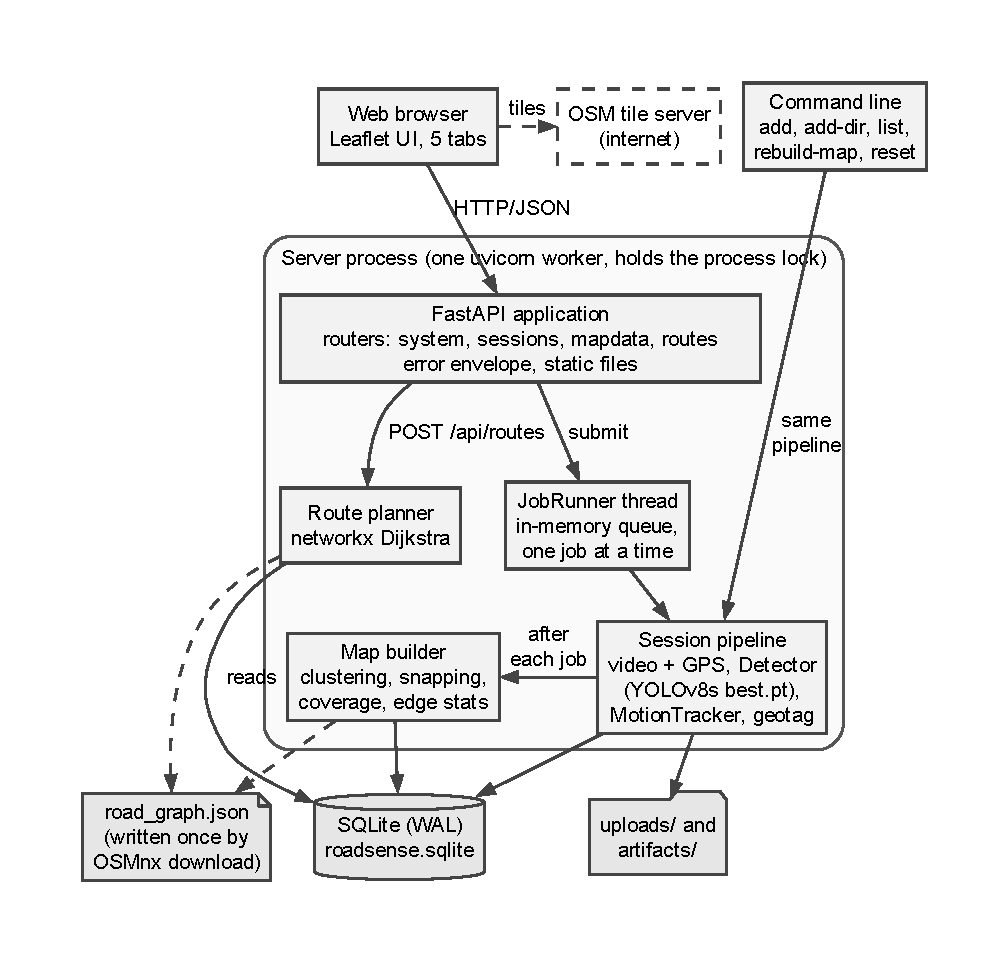
\includegraphics[width=0.68\textwidth]{ch4_architecture.pdf}
\caption{Runtime architecture. Solid arrows are calls or data flow; dashed arrows are read-only access or the optional base map.}
\label{fig:ch4-architecture}
\end{figure}

When it starts, the application uses the operating system to lock a file beside the database. A second server, or a command-line process that writes data, therefore cannot use the same database at the same time. Since no other process can own a job, any job still marked queued or running from an earlier run can safely be set to failed. A job whose detector fails on 2\% of the analysed frames or fewer is complete; up to 25\% it is kept as partial with a warning, and beyond that it fails and nothing is stored. Figure~\ref{fig:ch4-dataflow} traces a single recording from upload through to the map.

\begin{figure}[!htbp]
\centering
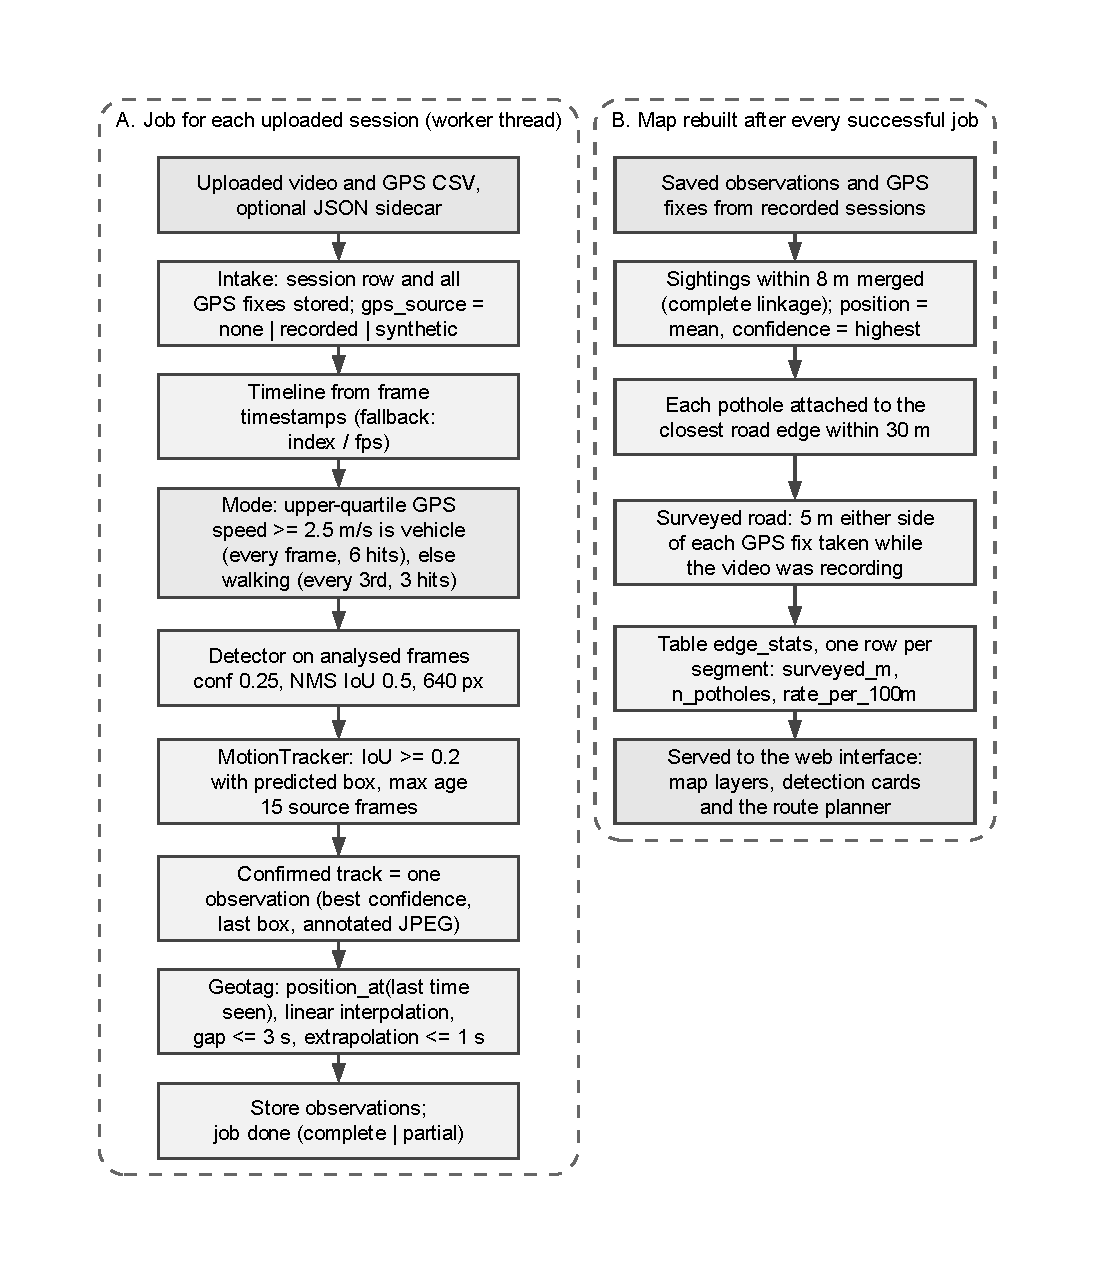
\includegraphics[width=0.62\textwidth]{ch4_dataflow.pdf}
\caption{How an uploaded video and GPS log become mapped potholes and road-segment statistics. Part A is the job run for each session and part B the map rebuild; the parameter values shown are the application defaults.}
\label{fig:ch4-dataflow}
\end{figure}

\subsection{Database structure}\label{sec:ch4-db}
All data lives in one SQLite file. It uses write-ahead logging and enforced foreign keys, and its schema carries a version number, currently 2, with no migration scripts between versions. Figure~\ref{fig:ch4-er} shows its nine tables. Four hold raw data: \texttt{sessions}, \texttt{gps\_fixes}, \texttt{jobs} and \texttt{observations} (one confirmed track with its best confidence, box, image and camera position). Four hold derived data that every map build wipes and recomputes: \texttt{builds}, \texttt{potholes}, \texttt{edge\_coverage} and \texttt{edge\_stats}. The table \texttt{meta} holds settings. A road segment is identified by its two OpenStreetMap node identifiers and edge key; because these are only meaningful for one graph, each build records the graph hash and routing refuses a build made with another graph.

\begin{figure}[!htbp]
\centering
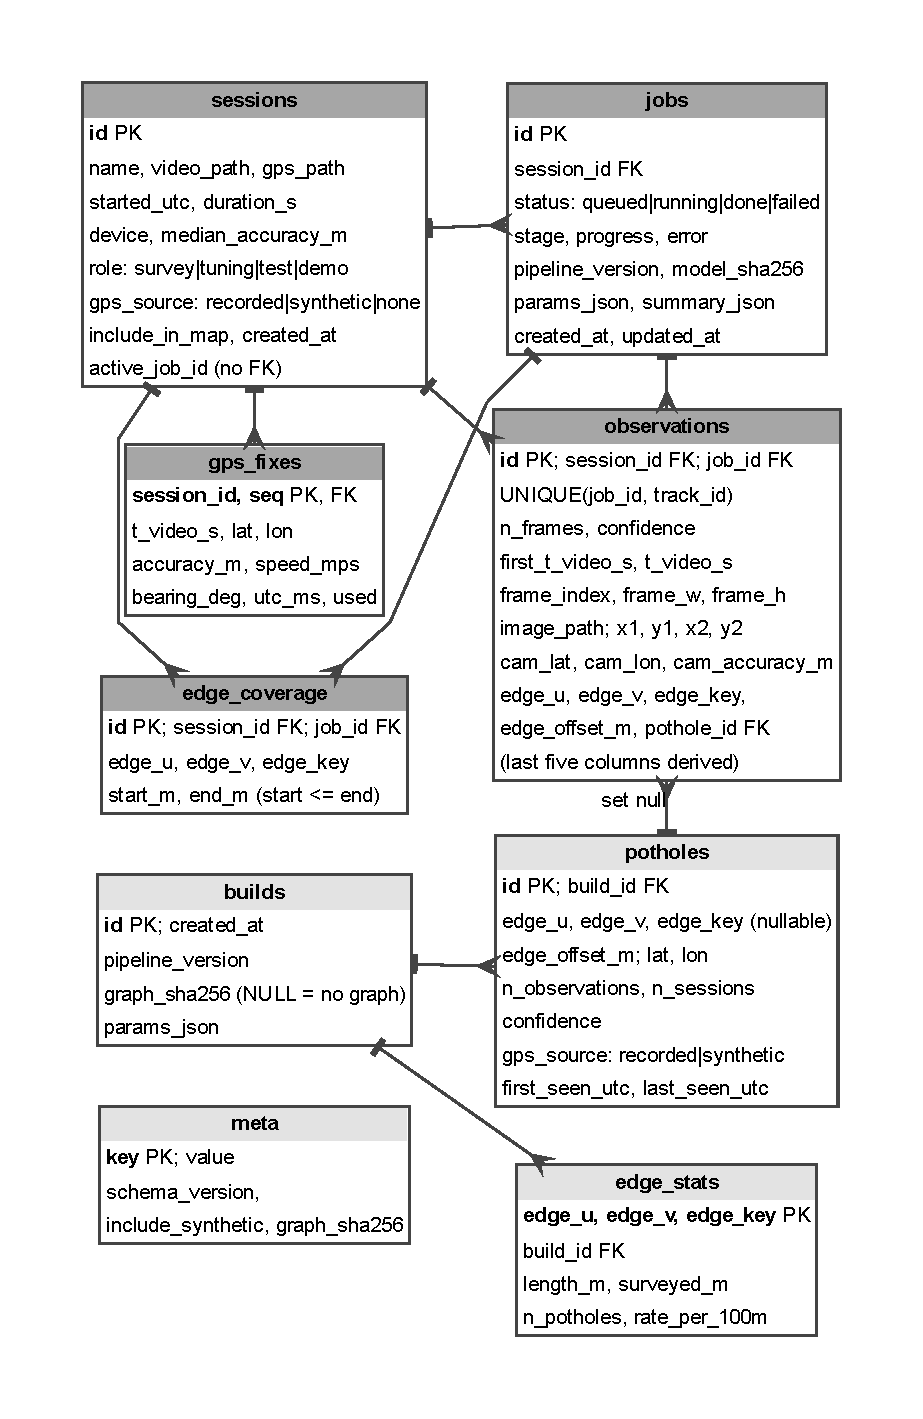
\includegraphics[width=0.55\textwidth]{ch4_er.pdf}
\caption{Entity-relationship diagram. Dark headers are raw tables; light headers are derived and control tables.}
\label{fig:ch4-er}
\end{figure}

\section{Use-case Diagram}\label{sec:ch4-usecase}
The system has no user accounts. Figure~\ref{fig:ch4-usecase} shows three actors: the user of the web interface, any other HTTP client (which can perform the same operations, since the interface calls only documented endpoints), and a person at the machine who uses the command line to add recordings, list sessions, rebuild the map or reset the database.

\begin{figure}[!htbp]
\centering
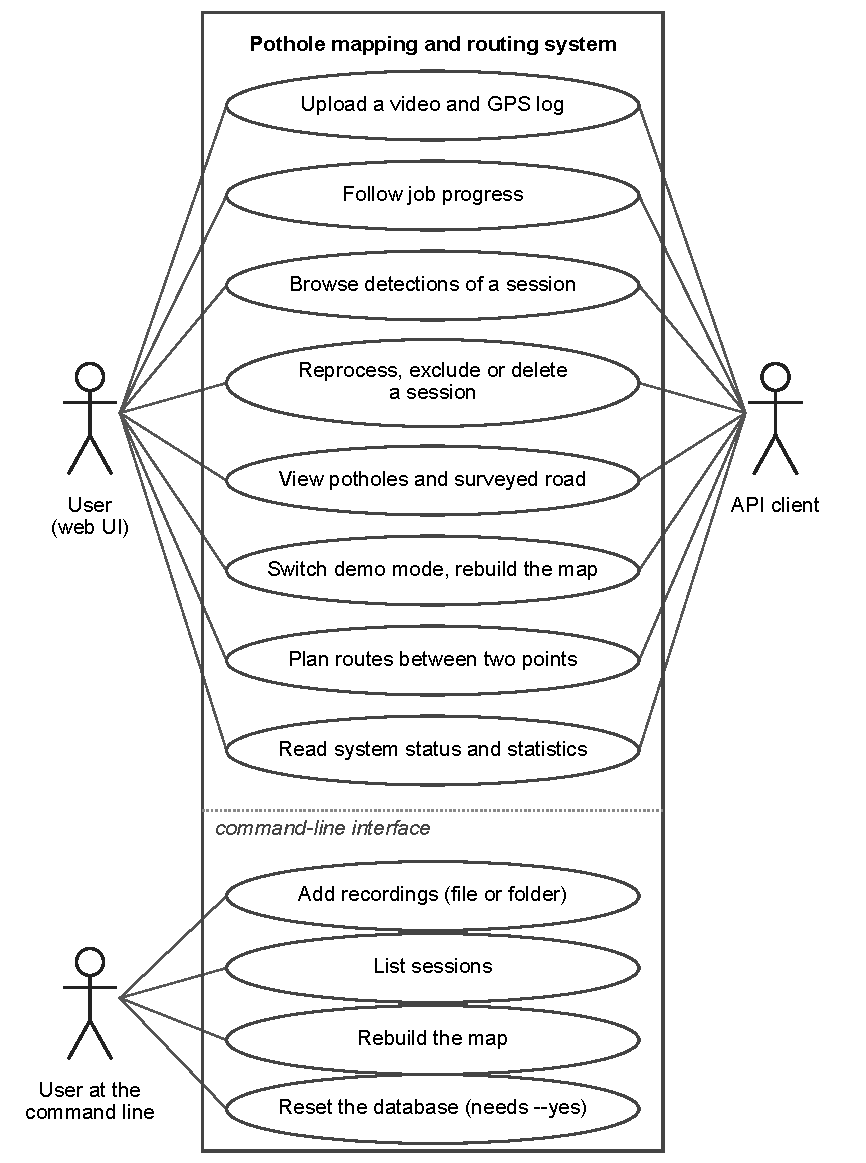
\includegraphics[width=0.58\textwidth]{ch4_usecase.pdf}
\caption{Use-case diagram. The web interface is itself a client of the API.}
\label{fig:ch4-usecase}
\end{figure}

\section{Class Diagram}\label{sec:ch4-class}
Most of the code consists of plain functions and small data classes rather than deep class hierarchies. Figure~\ref{fig:ch4-class-pipeline} covers the detection pipeline. For each job, the runner calls \texttt{process\_session}, which picks a tracking plan, runs the detector over the sampled frames and hands the detections to a \texttt{MotionTracker}. The pipeline talks to the detector only through the \texttt{DetectorLike} protocol. In normal use the \texttt{Detector} class fulfils it with an Ultralytics model, while the tests plug in a fake detector instead. On the service side, \texttt{EdgeIndex} snaps points onto road edges, and both the map builder and \texttt{plan\_routes} are functions that read the road graph and the database.

\begin{figure}[!htbp]
\centering
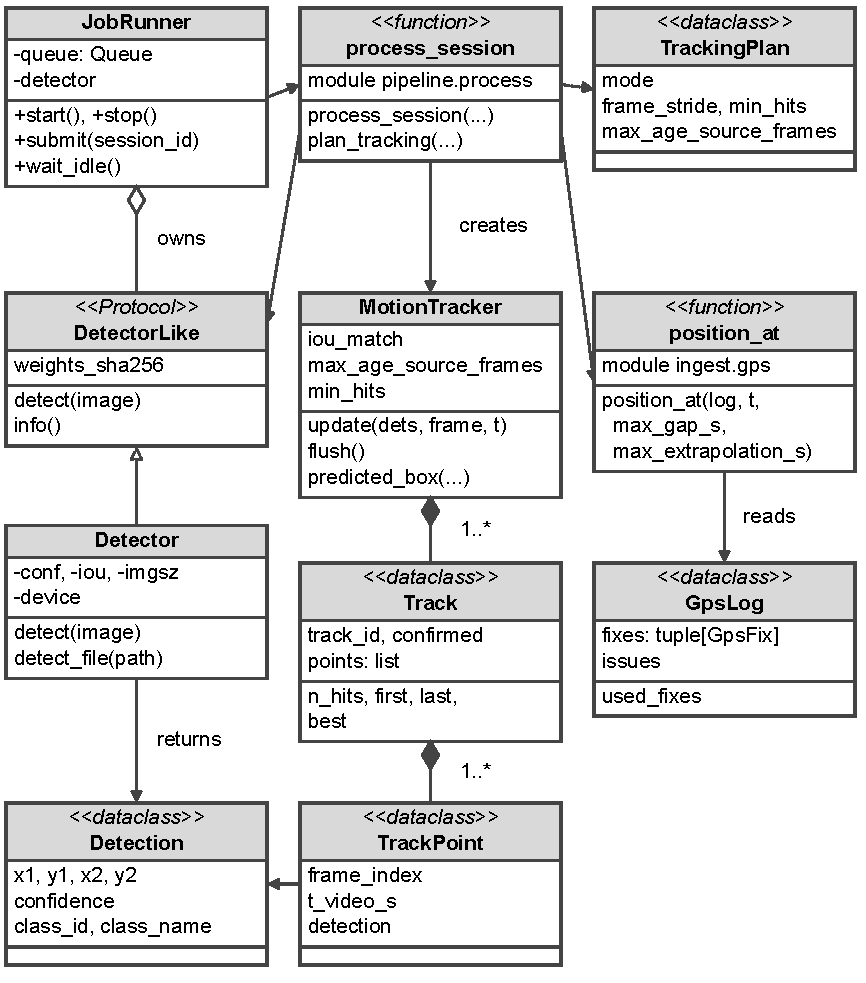
\includegraphics[width=0.66\textwidth]{ch4_class_pipeline.pdf}
\caption{Classes and function modules of the detection pipeline.}
\label{fig:ch4-class-pipeline}
\end{figure}

\section{Sequence Diagram}\label{sec:ch4-seq}
Figure~\ref{fig:ch4-seq-upload} follows an upload. Before replying with status 202, the API has already saved the session and its GPS fixes and created the job, so detection never happens inside the request itself. From then on the browser asks for the job status once a second. Meanwhile the worker runs the pipeline, saves the observations and the job status in a single transaction, and rebuilds the map. A route request, by contrast, is answered straight away from the stored map.

\begin{figure}[!htbp]
\centering
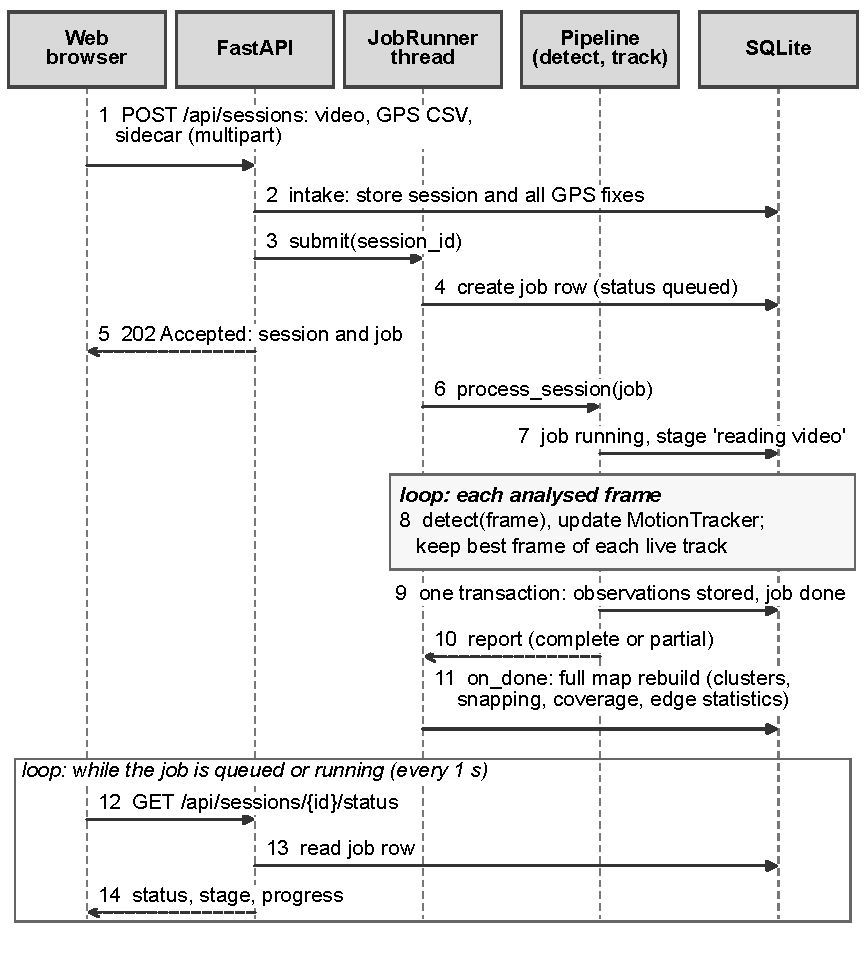
\includegraphics[width=0.72\textwidth]{ch4_seq_upload.pdf}
\caption{Sequence diagram for uploading and processing a session.}
\label{fig:ch4-seq-upload}
\end{figure}

\section{Detection-to-Map Pipeline Design}\label{sec:ch4-pipeline}

\subsubsection*{Sampling mode}
The upper quartile of the GPS speeds in the session decides the mode. At 2.5 m/s or more the session is a vehicle recording: every frame is analysed and a track needs 6 detections to be confirmed. Otherwise every third frame is analysed and 3 detections suffice. The upper quartile is used so that a ride with long stops is still treated as a vehicle recording.

\subsubsection*{Motion-aware tracker}
At vehicle speed a pothole can move further between analysed frames than its own height, so its boxes in consecutive frames may not overlap. The tracker therefore predicts each live track's box by shifting its last box by the track's average centre velocity over up to its last six points, and matches detections to predicted boxes greedily by intersection over union (IoU) of at least 0.2. A track ends after 15 source frames without a match; a track with enough hits becomes one observation. It is a simple tracker with no Kalman filter or appearance model, chosen over ByteTrack \cite{zhang2022bytetrack} to avoid an extra dependency.

\subsubsection*{Geotagging}
An observation is positioned at the camera location at the time $t$ the track was last seen, by linear interpolation between the bracketing GPS fixes at times $t_a \le t \le t_b$ with positions $p_a$ and $p_b$:
\begin{equation}
p(t)=p_a+\frac{t-t_a}{t_b-t_a}\,(p_b-p_a).
\label{eq:ch4-interp}
\end{equation}
No position is returned if the fixes are more than 3 s apart, and fixes with accuracy worse than 25 m are not used. No forward offset is applied, so a mapped pothole lies a few metres behind its true position, plus GPS error.

\subsubsection*{De-duplication and snapping}
Sightings from several tracks or passes are merged by greedy complete linkage: a set of sightings forms one mapped pothole only if every pair is within 8 m. Complete linkage replaced single linkage, which chained a line of sightings into one long pothole. Each mapped pothole is then snapped to the nearest road edge within 30 m; snapping is per point, so it can choose the wrong one of two close parallel roads.

\subsubsection*{Surveyed length}
A segment counts as surveyed only where a recorded session's GPS trace, clipped to the video interval, actually ran: each fix covers 5 m on either side, and consecutive fixes at most 3 s apart fill the span between them. For each edge the builder stores the surveyed length $s$, the number of mapped potholes $n$ and the rate $100\,n/s$ potholes per 100 m.

\section{Route-cost Design}\label{sec:ch4-route}
Road that has not been surveyed is unknown, not clean. For a directed edge of length $L$ metres with $n$ mapped potholes and $s$ surveyed metres, the router estimates the expected potholes as
\begin{equation}
E=n+r\,\frac{L-s}{100},
\qquad
r=\frac{100\,N+r_0\,\psi}{S+\psi},
\label{eq:ch4-expected}
\end{equation}
where $r$ is the assumed rate per 100 m on unsurveyed road, $N$ and $S$ are the mapped on-road potholes and surveyed metres over the whole map, and $r_0=1.0$ per 100 m and $\psi=500$ m are stated assumptions. The rate starts at $r_0$ and moves toward the observed rate as more road is surveyed, so one pothole on a few metres cannot produce an extreme value. The cost of the edge for an avoidance setting $a\in[0,1]$ is
\begin{equation}
\mathrm{cost}=L+a\,\lambda\,E,\qquad \lambda=300\ \mathrm{m},
\label{eq:ch4-cost}
\end{equation}
so at $a=1$ the router accepts a 300 m detour to avoid one expected pothole. The cost has no severity, confidence weighting or traffic term.

The router runs Dijkstra's algorithm \cite{dijkstra1959note} three times, for $a=0$ (Shortest), the user's setting, and $a=1$ (Strongest pothole avoidance), and merges identical routes, so it returns one to three routes. For each it reports the distance, a travel time from speed limits, the mapped potholes passed, the surveyed share $f$ of its length, and an evidence level: adequate if $f\ge0.8$, partial if $0.2\le f<0.8$ and insufficient otherwise. These thresholds, like $r_0$, $\psi$ and $\lambda$, are configuration values that have not been validated. Generated text never calls a road safe, clear or pothole-free. Figure~\ref{fig:ch4-routecost} shows the computation.

\begin{figure}[!htbp]
\centering
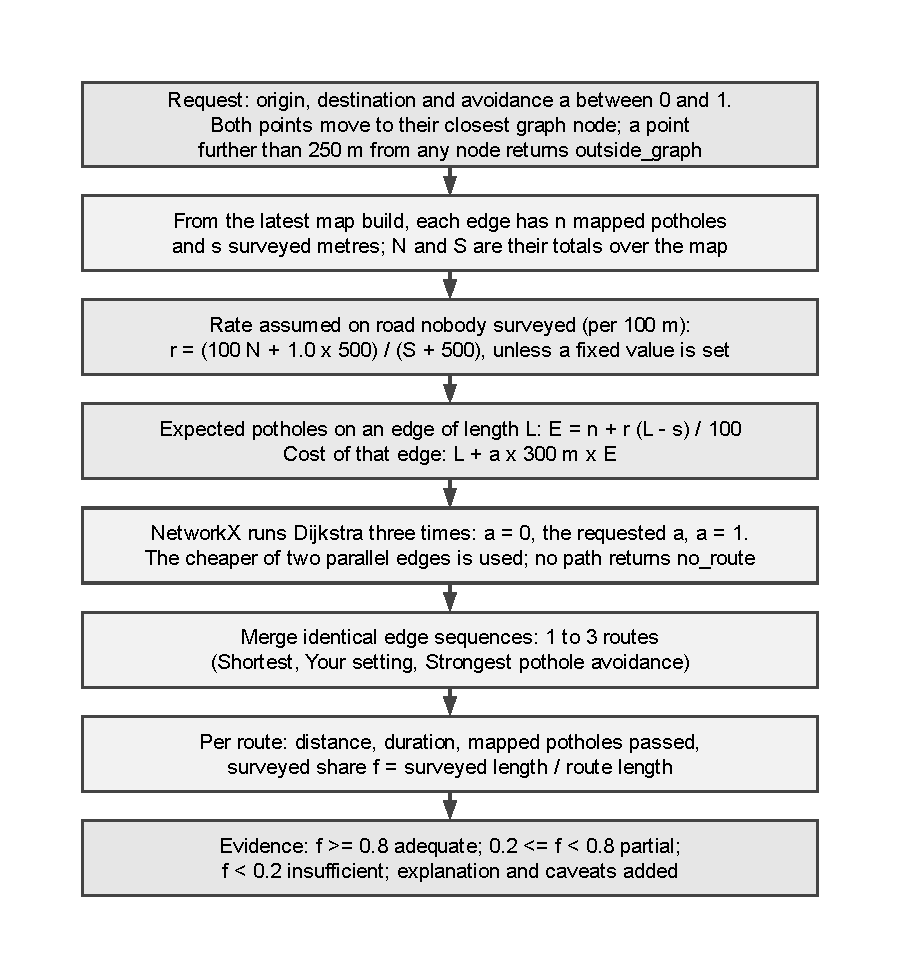
\includegraphics[width=0.5\textwidth]{ch4_routecost.pdf}
\caption{Route-cost computation from a request to a route plan.}
\label{fig:ch4-routecost}
\end{figure}

\section{Dataset Preparation Design}\label{sec:ch4-dataset}
The deployed baseline is trained on single-class RDD2022 \cite{arya2022rdd2022}; the experimental candidate adds HRP4K \cite{chen2026hrp4k}; a third dataset \cite{giordani2026roaddamage} is kept for evaluation only. The pipeline in Figure~\ref{fig:ch4-datasetpipe} is designed around one risk, leakage between training and evaluation data \cite{barz2020train,roberts2017crossvalidation}.

\begin{figure}[!htbp]
\centering
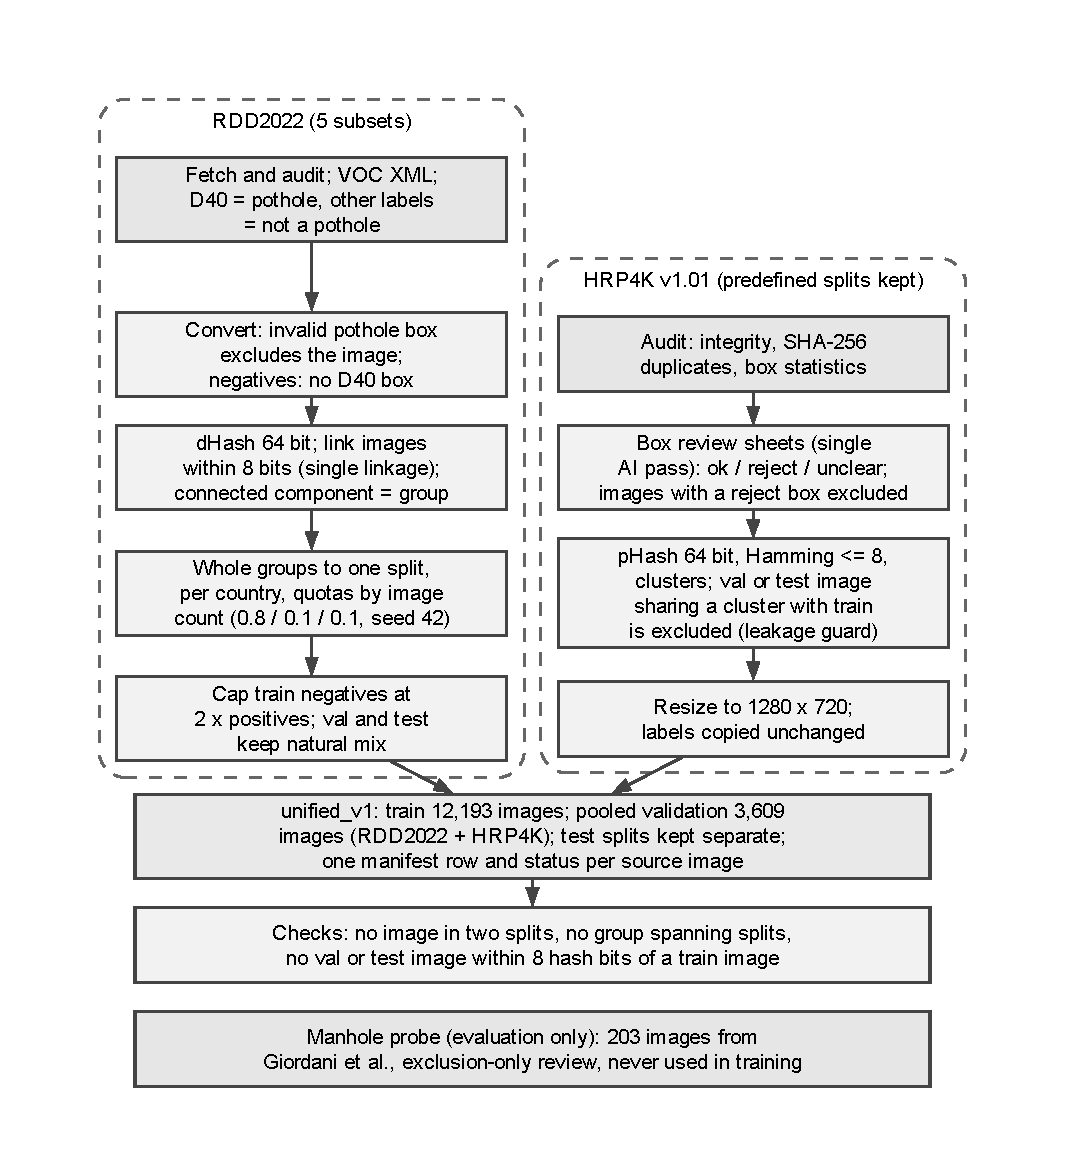
\includegraphics[width=0.68\textwidth]{ch4_datasetpipe.pdf}
\caption{Design of the dataset preparation pipeline.}
\label{fig:ch4-datasetpipe}
\end{figure}

In RDD2022 only the label D40 is a pothole; an image is positive if it has at least one D40 box and negative otherwise. Images are grouped by a 64-bit perceptual hash \cite{zauner2011rihamark}: two images of the same country are linked when their hashes differ in at most 8 bits, the connected components are the groups, and whole groups are assigned to the training, validation and test splits (80/10/10, seed 42). Grouping replaced an earlier split by blocks of image identifiers, which leaked because the identifiers are not in capture order. HRP4K keeps its predefined split, and a leakage guard removes any validation or test image that shares a hash cluster with a training image. Label review follows an exclusion-only rule: images may be removed, but boxes are never edited, added or relabelled. The same groups serve as the resampling units of the bootstrap (Section~\ref{sec:ch6-protocol}).

\section{Detector Architecture}\label{sec:ch4-yolo}
The detector is YOLOv8s \cite{jocher2023yolov8}, a single-stage detector of the YOLO family \cite{redmon2016yolo}, with one output class and 11,135,987 parameters. Figure~\ref{fig:ch4-yolov8s} shows its structure as defined in Ultralytics 8.4.210. The backbone downsamples the image to strides 8, 16 and 32 using C2f blocks, which build on the cross-stage partial idea \cite{wang2020cspnet}, and ends with a fast spatial pyramid pooling block. The neck fuses the three scales along top-down and bottom-up paths \cite{lin2017fpn,liu2018panet}, giving $80\times80$, $40\times40$ and $20\times20$ output maps at 640 px. The anchor-free head predicts boxes as distributions over the distances to the four sides \cite{li2020generalized} and one class logit per location, and training assigns positives with a task-aligned assigner \cite{feng2021tood}. Training starts from COCO-pretrained weights \cite{lin2014coco}.

\begin{figure}[!htbp]
\centering
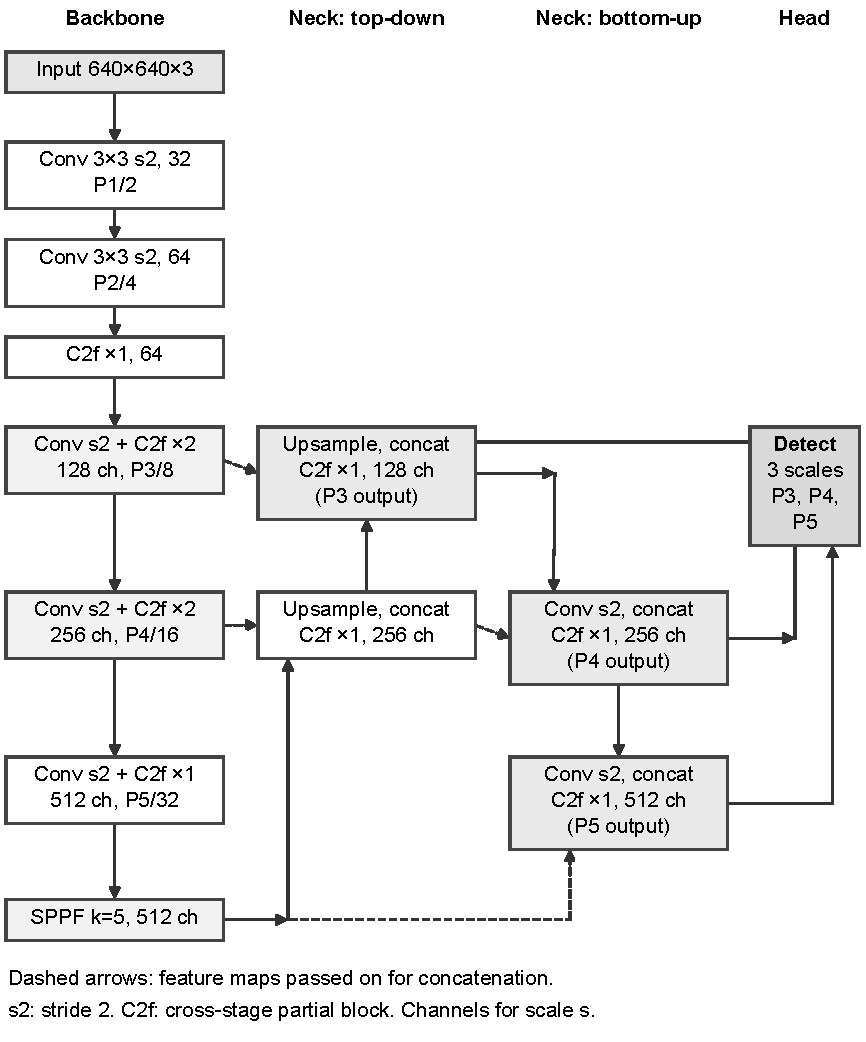
\includegraphics[width=0.62\textwidth]{ch4_yolov8s.pdf}
\caption{Structure of YOLOv8s with one class, drawn from the Ultralytics 8.4.210 model definition.}
\label{fig:ch4-yolov8s}
\end{figure}

\chapter{Implementation}\label{ch:implementation}

\section{Overview of Technologies Used}\label{sec:ch5-tech}
The application and the model-development tools are written in Python and installed as one package. Table~\ref{tab:ch5-tech} lists the main technologies with the versions in the development environment (Windows 11, RTX 4060 Laptop GPU). The training runs used a rented RTX 5090 under Linux with Python 3.12 and PyTorch 2.14.1 for CUDA 13.0.

\begin{table}[!htbp]
\centering
\small
\renewcommand{\arraystretch}{1.2}
\begin{tabular}{|L{3.6cm}|L{2.6cm}|L{6.8cm}|}
\hline
\textbf{Technology} & \textbf{Version} & \textbf{Use}\\
\hline
Python & 3.10.0 & Language of all code\\
\hline
PyTorch \cite{paszke2019pytorch} & 2.14.1 (CUDA 12.6) & Tensor library under Ultralytics\\
\hline
Ultralytics & 8.4.210 (pinned) & YOLOv8s training, validation and inference\\
\hline
OpenCV, NumPy, Pillow & 5.0.0.93, 2.2.6, 12.3.0 & Video decoding, array computation, image hashing\\
\hline
pydantic, PyYAML & 2.14.3, 6.0.3 & Strictly validated YAML configuration\\
\hline
FastAPI, uvicorn & 0.162.4, 0.54.0 & REST API, static files, server (one worker)\\
\hline
SQLite (\texttt{sqlite3}) & standard library & Storage in write-ahead logging mode, plain SQL\\
\hline
OSMnx \cite{boeing2017osmnx}, NetworkX & 2.0.7, 3.4.2 & One-off road-network download; graph and Dijkstra\\
\hline
Leaflet & 1.9.4 & Interactive map in the browser\\
\hline
pytest, httpx & 9.1.1, 0.28.1 & Test suite and API test client\\
\hline
\end{tabular}
\caption{Main technologies and their use.}
\label{tab:ch5-tech}
\end{table}

\section{Implementation details of modules}\label{sec:ch5-modules}

\subsection{Dataset tooling}\label{sec:ch5-datatools}
The package \texttt{roadsense.data} downloads RDD2022 from its figshare record with an MD5 check, parses the Pascal VOC annotations, keeps the label D40 as the only pothole class and writes YOLO label files together with a manifest that gives every source image a status. An image with an invalid pothole box is excluded whole, since dropping only the box would turn a pothole image into a false negative. The split functions implement the hash grouping of Section~\ref{sec:ch4-dataset}, and an independent script re-derives the converted dataset from the raw XML to detect converter defects. The builder \texttt{scripts/build\_unified\_v1.py} produces the versioned datasets \texttt{unified\_v1} (RDD2022 and HRP4K) and \texttt{kaggle\_probe\_v1} (the evaluation-only manhole probe). The builder works in a temporary directory and moves the result into place only after its checks pass: every image must decode, no image may appear in two splits, and no group may be divided between splits. Running it twice on the same input produces the same manifests and labels.

\subsection{Training}\label{sec:ch5-training}
A model is trained by running the module \texttt{roadsense.training.train} with a configuration file given through the \texttt{-{}-config} option. The entry point validates the YAML configuration (unknown keys are errors), checks that the dataset defines exactly one class named pothole, refuses weights for other tasks, refuses any image under a directory named test, and writes the resolved configuration and dataset hashes into the run directory before training. Table~\ref{tab:ch5-train} compares the two runs.

\begin{table}[!htbp]
\centering
\small
\renewcommand{\arraystretch}{1.2}
\begin{tabular}{|L{3.3cm}|L{4.5cm}|L{5.0cm}|}
\hline
\textbf{Setting} & \textbf{Baseline (deployed)} & \textbf{Candidate (experimental)}\\
\hline
Initial weights & COCO-pretrained \texttt{yolov8s.pt} \cite{lin2014coco} & Baseline checkpoint (epoch 56)\\
\hline
Training data & RDD2022, 8,220 images & RDD2022 and HRP4K, 12,193 images\\
\hline
Validation data & RDD2022, 2,784 images & Pooled RDD2022 and HRP4K, 3,609 images\\
\hline
Image size & $640\times 640$ & $1280\times 1280$\\
\hline
Batch & 64 & 16 with 4 accumulation steps\\
\hline
Epochs & 100 (patience 20); stopped at 76, best 56 & 50; selected \texttt{epoch25.pt}\\
\hline
Optimiser, learning rate & Automatic choice (MuSGD), 0.01 & AdamW \cite{loshchilov2019adamw}, 0.001, cosine schedule\\
\hline
Augmentation & \multicolumn{2}{L{9.5cm}|}{Mosaic \cite{bochkovskiy2020yolov4} (off for the last 10 epochs), HSV jitter, translation 0.1, scale 0.5, horizontal flip; vertical flip off}\\
\hline
Seed & \multicolumn{2}{L{9.5cm}|}{42, deterministic mode, mixed precision}\\
\hline
Training time & 20 min 12 s & 78.98 min\\
\hline
\end{tabular}
\caption{Configurations of the baseline and candidate training runs.}
\label{tab:ch5-train}
\end{table}

The optimiser of the candidate was set explicitly because Ultralytics' automatic choice depends on the number of iterations; its learning rate was halved from the AdamW default of 0.002 because the weights were already trained for the task, a judgement that was not tuned. Patience equals the number of epochs so that Ultralytics' own stopping metric could not end the run early; checkpoints were saved every five epochs and selected afterwards (Section~\ref{sec:ch6-results}). Only one run exists for each configuration.

Both runs used a rented RTX 5090 on Vast.ai under a budget set by the project owner. A bundle builder packed only the training and validation images and lists (2.24 GB, with a content digest) and fails if any test path is involved; the bundle was uploaded with 16 parallel streams and verified remotely by SHA-256. On the rented machine, a script installed the pinned dependencies, checked the bundle, started training under a watchdog and packed up the results at the end. As a safety net it could also destroy the instance after 205 minutes. Before renting anything, we rehearsed the complete sequence in a Linux environment on the laptop.

\subsection{Evaluation tooling}\label{sec:ch5-eval}
The protocol of Section~\ref{sec:ch6-protocol} is implemented in \texttt{scripts/eval\_checkpoint.py}. For each dataset it calls Ultralytics validation once, with the confidence floor set to 0.001, and saves the predictions. All metrics are then recomputed from that file with the script's own greedy matching and 101-point average precision, so a single pass covers every threshold. A select mode chooses the threshold on a validation list; an apply mode applies a stored threshold to a test list and refuses a checkpoint with a different hash, a different image size or images shared with the selection list. A comparison script computes paired bootstrap differences between two evaluations. A further script selects the candidate checkpoint by a rule written into its header before the run, and refuses test lists.

\subsection{Ingest, detection and tracking}
The ingest package reads video timestamps from OpenCV, using the presentation timestamps if they are finite and strictly increasing for the whole file and frame index divided by frame rate otherwise; the two are never mixed. The GPS parser reads a CSV file with time on the video clock, latitude, longitude, accuracy, speed and bearing, and records every rejected row with its line number and reason. \texttt{Detector} loads the Ultralytics model only when it is first needed, records the SHA-256 hash of the weights and runs on the GPU if one is available. It rejects any model whose class names are anything other than \{0: pothole\}, which stops generic pretrained weights from being loaded by accident. Tracking is handled by \texttt{MotionTracker} (Section~\ref{sec:ch4-pipeline}), which always gives the same output for the same input. For every track the pipeline keeps only the annotated frame with the most confident detection and compresses it to JPEG straight away, so memory use does not grow.

\subsection{Building the map and planning routes}
The clustering code in \texttt{geo/dedup.py} places points on a grid in a local projection, so that it only has to compare neighbouring cells. It computes the great-circle distance for each candidate pair and merges clusters only under the complete-linkage rule. Road snapping is done by \texttt{EdgeIndex}, which holds every undirected road edge as a polyline in local metres and finds the nearest one with vectorised NumPy operations. The function \texttt{rebuild\_map} recomputes all derived tables in one write transaction, retried if the database is locked, and each build records the jobs, settings, code version and graph hash it used.

The road graph is downloaded once with OSMnx as the drivable OpenStreetMap network of a bounding box \cite{haklay2008osm} and stored as JSON with its hash. The project's graph covers about 4 by 3.4 km of Bengaluru with 2,996 nodes and 7,138 directed edges. Routing follows Section~\ref{sec:ch4-route}. \texttt{plan\_routes} passes a callable edge weight to the NetworkX shortest-path function, so the search it runs is Dijkstra's algorithm. A returned route includes its geometry, divided into surveyed, demonstration and unsurveyed stretches, together with its figures and a short explanation in plain language. It also carries fixed caveats saying that potholes the detector missed, or that lie on unsurveyed road, are not counted, and that severity is not recorded.

\subsection{Backend services}
The FastAPI application is split into four routers. The web files are mounted last so that they can never hide an API route, and every error comes back in the same format, with a code and a message. Table~\ref{tab:ch5-api} lists the 20 endpoints. When a video is uploaded, the endpoint copies it in chunks and counts the bytes as it goes, stopping at the 2,048 MB limit, before it creates the session and queues the job. \texttt{JobRunner} manages one worker thread and its in-memory queue, and no SQLite connection is ever shared between threads. \texttt{ProcessLock} holds a non-blocking operating-system lock on a file beside the database, and the operating system frees that lock however the process exits.

\begin{table}[!htbp]
\centering
\small
\renewcommand{\arraystretch}{1.2}
\begin{tabular}{|L{2.4cm}|L{5.6cm}|L{5.0cm}|}
\hline
\textbf{Group} & \textbf{Endpoints} & \textbf{Purpose}\\
\hline
System (3) & \texttt{GET /api/health}, \texttt{/api/system}, \texttt{/api/stats} & Liveness, versions and model hash, counts\\
\hline
Sessions (10) & \texttt{POST/GET /api/sessions}, \texttt{GET/PATCH/DELETE /api/sessions/\{id\}}, \texttt{.../status}, \texttt{.../reprocess}, \texttt{.../detections}, \texttt{.../track}, \texttt{GET /api/artifacts/\{path\}} & Upload (202 with job), job status, observations, GPS track, images, include or delete\\
\hline
Map (4) & \texttt{GET /api/potholes}, \texttt{/api/potholes/\{id\}}, \texttt{/api/coverage}, \texttt{POST /api/map/rebuild} & Mapped potholes and surveyed road in a bounding box; rebuild\\
\hline
Routing (3) & \texttt{GET /api/routes/info}, \texttt{POST /api/routes}, \texttt{GET /api/demo/route-example} & Cost settings; plan one to three routes; demonstration route\\
\hline
\end{tabular}
\caption{HTTP endpoints grouped by purpose.}
\label{tab:ch5-api}
\end{table}

\subsection{User interfaces}
The browser interface is written in plain HTML, CSS and JavaScript modules, uses Leaflet 1.9.4 for the map and needs no build step. It is organised into five tabs. The dashboard shows summary statistics and a switch for demonstration mode, and the upload tab is a form for the video and GPS files. The sessions tab lists recordings with their job progress and lets the user reprocess or delete them. In the detections tab every observation appears as a card with its annotated frame. The route planner takes an origin and a destination, has an avoidance slider running from 0 to 1, and shows each route as a card with its surveyed share and evidence level. On the map, recorded potholes, demonstration potholes and surveyed road are separate layers, and a banner is shown whenever demonstration mode is active. Outside the browser, a command-line program offers the commands \texttt{add}, \texttt{add-dir}, \texttt{list}, \texttt{rebuild-map} and \texttt{reset}, and any command that writes data takes the process lock first. A script creates one synthetic demonstration session from RDD2022 validation images with a generated GPS trace, captioned and flagged as synthetic.

\section{Challenges encountered and Strategies used to tackle}\label{sec:ch5-challenges}

\subsubsection*{Near-duplicate leakage}
The first split assigned blocks of consecutive image identifiers, assuming capture order. A scan showed that the identifiers are shuffled: under a block split 17.6\% of India's validation images had a training image within 4 bits of hash distance. Perceptual-hash grouping replaced it, and for HRP4K, where a difference hash put 4,250 of 6,003 images into one component, a DCT-based hash and a leakage guard were used instead.

\subsubsection*{Thresholds selected on test data}
The summary precision and recall that Ultralytics reports are computed at the confidence that maximises F1 on the evaluated split itself, which on a test split selects the operating point on test data. We rewrote the evaluation so that thresholds are selected on validation data and applied unchanged to test data; the library's summary values are not used in this report.

\subsubsection*{An average-precision discrepancy}
The first version of our script closed the precision-recall curve differently from Ultralytics, which inflated AP on low-recall sets such as HRP4K for the baseline. We corrected it and marked the earlier results as superseded; afterwards our mAP\textsubscript{50} agreed with the library value to within 0.0014.

\subsubsection*{A baseline nearly blind on forward-view footage}
The RDD2022 baseline detects almost nothing on HRP4K (validation recall 0.051 at its threshold), partly because the median HRP4K pothole is about 10 px at 640 px input. The response was the candidate experiment, whose results and limits are in Chapter~\ref{ch:results}.

\subsubsection*{Cloud resources}
The first baseline attempt with 12 data-loader workers was killed by the container memory limit, because Ultralytics starts additional validation workers; the run with 6 workers completed. The slow single-stream upload led to the parallel chunked upload.

\subsubsection*{Track fragmentation at vehicle speed}
The first tracker compared each detection with a track's last box, so at vehicle speed one pothole became several short tracks that were discarded. Sampling every frame for vehicle sessions, predicting boxes from track velocity and measuring track age in source frames fixed this in replays of saved detections, which show continuity only, not accuracy.

\subsubsection*{Sparse coverage for routing}
Our recordings cover about 1,020 m on seven disconnected stretches, so a real route comparison is impossible. Route recommendation is demonstrated on a synthetic session, with safeguards so that it cannot be mistaken for data: demonstration mode is off by default, synthetic and recorded sightings are clustered separately, surveyed-road figures use recorded sessions only, and the interface labels demonstration data.

\chapter{Testing and Experimental Analysis and Results}\label{ch:results}

This chapter reports the automated tests of the software, the experimental datasets, the evaluation of the deployed baseline and the experimental candidate, and a qualitative comparison with the earlier implementation on our own recordings.

\section{Unit Testing}\label{sec:ch6-tests}
The software is tested with pytest. The suite has 1,101 tests in 45 test files. In the full configuration, which includes the tests that load the real checkpoint and use the GPU, all 1,101 tests passed in 115.80 s on the development laptop (Windows 11, Python 3.10.0, pytest 9.1.1, RTX 4060 Laptop GPU), with one deprecation warning; a repeated full run also passed. A fast subset that uses a fake detector and needs no GPU is selected with \texttt{pytest -m "not slow"}. Table~\ref{tab:ch6-test-counts} gives the tests by area.

\begin{table}[!htbp]
\centering
\small
\renewcommand{\arraystretch}{1.2}
\begin{tabular}{|L{4.4cm}|L{7.4cm}|r|}
\hline
\textbf{Area} & \textbf{Examples of what is checked} & \textbf{Tests} \\
\hline
Video and GPS ingestion & GPS row rejection, clipping a trace to the video, timestamps & 241 \\
\hline
Detection, tracking, pipeline & A box moving faster than its own height stays one track; short blips rejected & 112 \\
\hline
Geospatial and map building & Complete linkage cannot grow a cluster past 8 m; snapping limit & 109 \\
\hline
Road graph and routing & Detour taken only when cheaper than the pothole penalty & 110 \\
\hline
Storage and process lock & Interrupted jobs marked failed; a second lock is refused & 37 \\
\hline
API, CLI, configuration, demo & Upload limits and error codes; demo data ignored when demo mode is off & 172 \\
\hline
ML and data tooling & Conversion edge cases, leakage guard, checkpoint selection ties, AP matches Ultralytics & 320 \\
\hline
\multicolumn{2}{|r|}{\textbf{Total}} & \textbf{1,101} \\
\hline
\end{tabular}
\caption{Automated tests by area, from the pytest collection of the full suite.}
\label{tab:ch6-test-counts}
\end{table}

Most tests target one function with small inputs built in the test. One metric test guards the average-precision correction described in Section~\ref{sec:ch5-challenges}: it checks that our AP routine agrees with the Ultralytics routine on a low-recall case. Two parts are covered only indirectly: the training entry point by configuration and dry-run tests, and the evaluation scripts by unit tests of their logic.

\section{Integration Testing}
Integration tests exercise several modules together with real components other than the detector. The API tests (79) run the application through the FastAPI test client on a temporary database with a fake detector, covering upload, the job runner, status, detections, map and coverage queries, routing, the error envelope and upload limits (a 3 MB file against a 1 MB limit must return 413 and leave nothing behind). The pipeline tests write small synthetic videos with moving objects and run the complete session processing. The map-building tests run the full derived-data rebuild, and the process-lock tests check that a second server on the same database cannot disturb the live server's jobs. Detector tests and tests marked slow load the real checkpoint.

Three things are not covered. The browser interface has no JavaScript or UI behaviour tests; only two tests check that the page is served with the right cache headers. No test measures end-to-end accuracy on labelled video from our roads, because none exists. Load behaviour is not tested.

\section{Experimental Dataset}\label{sec:ch6-data}
Table~\ref{tab:ch6-sources} lists the three public datasets. For RDD2022 we used five subsets (India, Japan, Czech Republic, United States, China MotorBike), 27,823 labelled images; China Drone was left out as not forward-facing and Norway because its very wide frames would shrink potholes to a few pixels at 640 px. The official RDD2022 test images are unlabelled, so our RDD2022 test split is an internal split of labelled images. HRP4K images were resized from $3840\times2160$ to $1280\times720$, at which the median box (square root of its area) is 20.1 px. Figure~\ref{fig:ch6-hrp-examples} shows typical HRP4K frames.

\begin{table}[!htbp]
\centering
\small
\renewcommand{\arraystretch}{1.2}
\begin{tabular}{|L{2.5cm}|L{5.4cm}|L{2.8cm}|L{2.2cm}|}
\hline
\textbf{Dataset} & \textbf{Origin} & \textbf{Licence as found} & \textbf{Role} \\
\hline
RDD2022 & Arya et al.\ \cite{arya2022rdd2022}; figshare record & CC BY 4.0 / CC BY-SA 4.0 & train, val, test \\
\hline
HRP4K v1.01 & Chen et al.\ \cite{chen2026hrp4k}; Zenodo record \cite{chen2026hrp4kzenodo} & CC BY 4.0 (metadata) & train, val, test (candidate) \\
\hline
Manhole probe & Giordani et al.\ \cite{giordani2026roaddamage}, via a Kaggle mirror & Not verified & evaluation only \\
\hline
\end{tabular}
\caption{Datasets used in the experiments.}
\label{tab:ch6-sources}
\end{table}

\begin{figure}[!htbp]
\centering
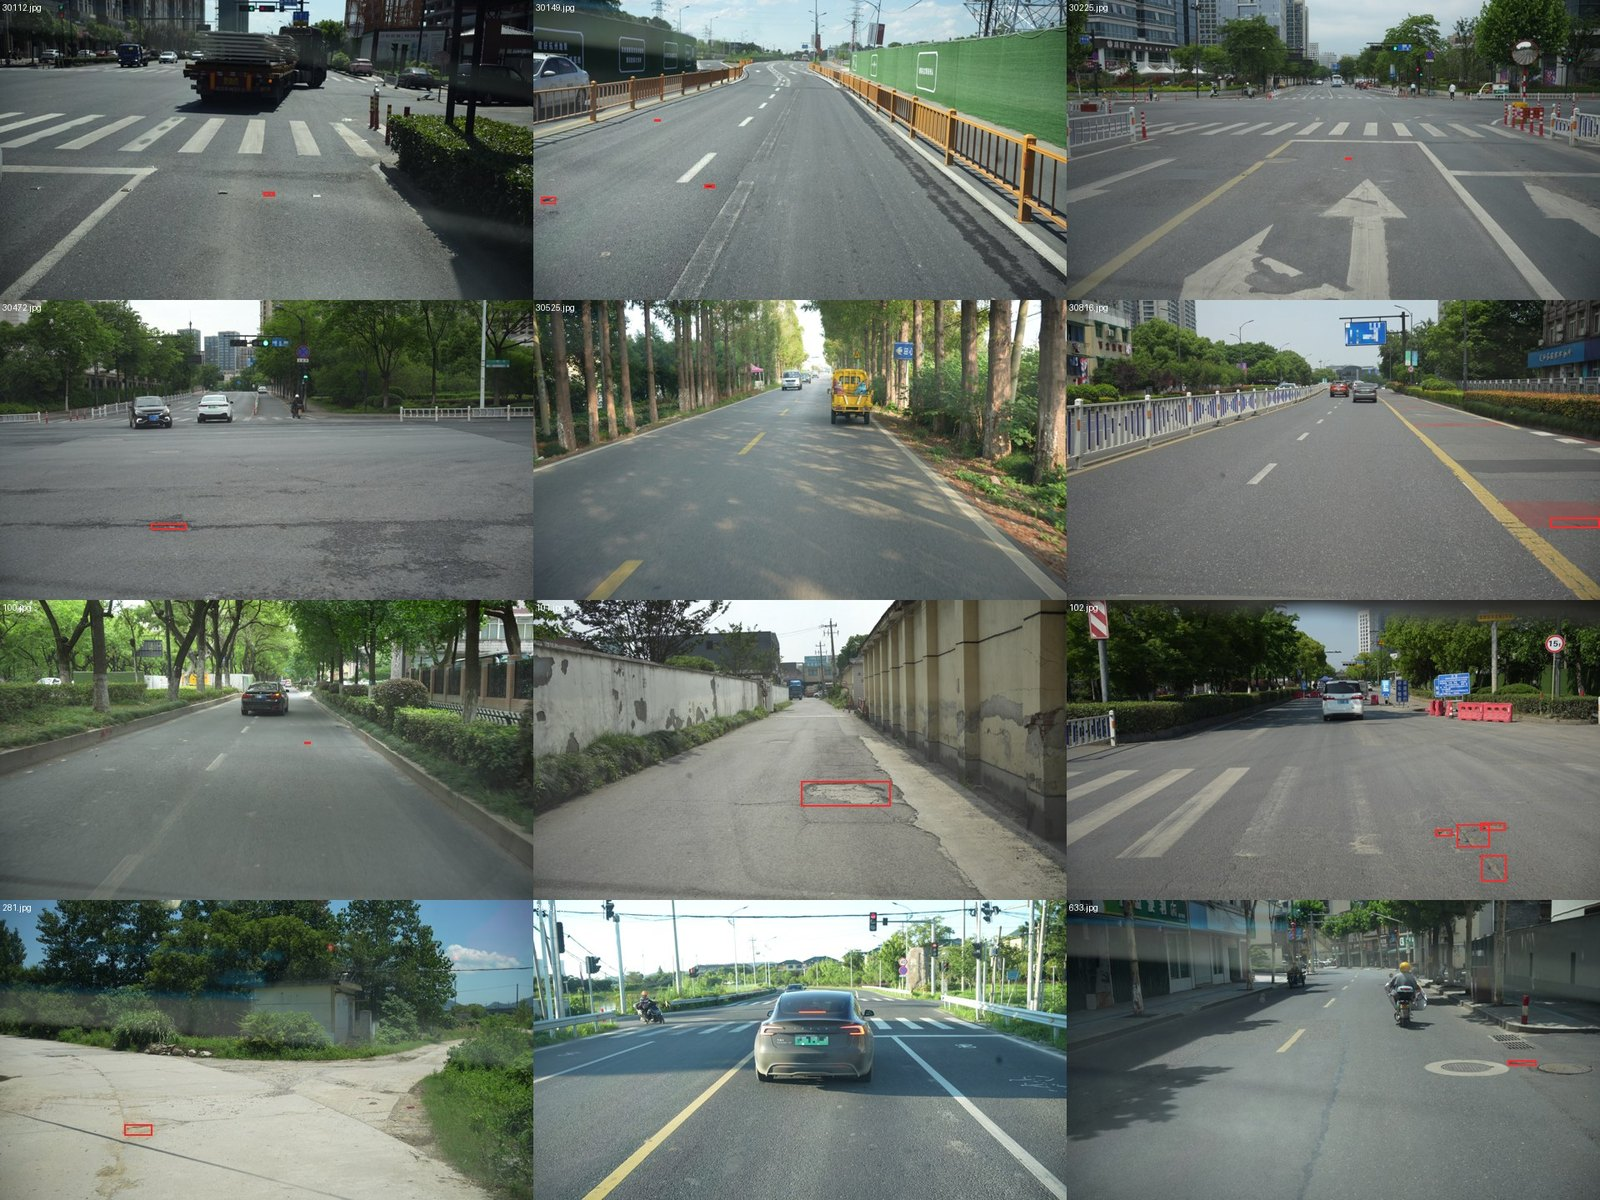
\includegraphics[width=0.55\textwidth]{ch6_hrp4k_examples.jpg}
\caption{HRP4K examples with the published boxes in red. Many potholes are only a few pixels wide at this scale. Source: HRP4K \cite{chen2026hrp4k}, CC BY 4.0 per the Zenodo metadata.}
\label{fig:ch6-hrp-examples}
\end{figure}

\subsubsection*{Review and exclusions}
The HRP4K labels were reviewed box by box in a single pass by an AI model over rendered tile sheets: of 7,217 boxes, 2,644 were judged ok, 400 rejected and 4,173 unclear. Under the exclusion-only rule, unclear boxes were kept and images with a clearly wrong box (a cover, kerb, marking, crack or patch) were excluded whole. There was no second reviewer and no agreement measure, so label noise remains: in a visual sample of 120 positive images, only about 92 of roughly 212 boxes clearly lay on a pothole. The manhole probe was reviewed more strictly and keeps 42 images with potholes plus 161 pothole-free images that each contain an intact manhole; its false-alarm rate therefore measures behaviour on manholes, not general behaviour.

\subsubsection*{Splits and leakage}
After grouping (Section~\ref{sec:ch4-dataset}), no group spans two splits and no validation or test image has a training image within 8 bits. The HRP4K leakage guard removed 51 validation and 76 test images. Some overlap remains: about 64\% of RDD2022 validation and test images have a training image at 9 to 12 bits, mostly similar road layouts rather than the same scene, so RDD2022 scores are probably optimistic for unseen roads. Training negatives in RDD2022 were capped at two per positive image; validation and test keep their natural mix (about 11\% positive). Table~\ref{tab:ch6-composition} gives the final composition.

\begin{table}[!htbp]
\centering
\small
\renewcommand{\arraystretch}{1.2}
\begin{tabular}{|L{2.8cm}|L{2.6cm}|r|r|r|r|}
\hline
\textbf{Source} & \textbf{Split} & \textbf{Images} & \textbf{Boxes} & \textbf{Positive} & \textbf{Empty} \\
\hline
RDD2022 & train & 8,220 & 5,017 & 2,740 & 5,480 \\
\hline
RDD2022 & validation & 2,784 & 477 & 299 & 2,485 \\
\hline
RDD2022 & test & 2,784 & 503 & 315 & 2,469 \\
\hline
HRP4K & train & 3,973 & 4,709 & 2,573 & 1,400 \\
\hline
HRP4K & validation & 825 & 922 & 535 & 290 \\
\hline
HRP4K & test & 811 & 836 & 538 & 273 \\
\hline
Manhole probe & evaluation only & 203 & 59 & 42 & 161 \\
\hline
\end{tabular}
\caption{Final composition of the experimental datasets. The probe also has 196 intact manhole boxes, which are not pothole targets.}
\label{tab:ch6-composition}
\end{table}

\section{Performance Analysis}

\subsection{Evaluation protocol}\label{sec:ch6-protocol}
A prediction matches a ground-truth box if their IoU is at least 0.5, greedily by descending confidence. At a confidence threshold $t$, precision $P=TP/(TP+FP)$, recall $R=TP/N_{gt}$ and
\begin{equation}
F_1=\frac{2PR}{P+R},
\label{eq:ch6-f1}
\end{equation}
where $N_{gt}$ is the number of ground-truth boxes. We also report false positives per image and mAP\textsubscript{50} and mAP\textsubscript{50--95} with the 101-point interpolation of Ultralytics \cite{padilla2020survey}. On the probe, the \emph{manhole hit share} is the fraction of the 196 manhole boxes overlapped (IoU $\ge 0.3$) by a pothole prediction.

The threshold of each model is the one that maximises $F_1$ on the pooled RDD2022 and HRP4K validation set, and it is applied unchanged to the test sets \cite{cawley2010overfitting}: 0.2705 for the baseline at 640 px and 0.2450 for the candidate at 1280 px. In the deployed application the confidence threshold is a provisional 0.25. The intervals come from a group bootstrap \cite{efron1993bootstrap}, in which whole near-duplicate groups are resampled 1,000 times and the 2.5th and 97.5th percentiles give the 95\% interval. Because both models are scored on the same resamples, their difference can be computed pair by pair \cite{koehn2004significance}, and an asterisk marks any interval that does not include zero. We did not correct for multiple comparisons. The test splits were also evaluated more than once during development, and no log of those evaluations was kept.

\subsection{Results of the baseline model}\label{sec:ch6-results}
Early stopping ended the baseline's training after 76 epochs, and we kept the checkpoint from epoch 56. Figure~\ref{fig:ch6-curves-baseline} shows the training-time curves on the RDD2022 validation split: the metrics flatten after about epoch 50 while the validation losses rise, a sign of overfitting.

\begin{figure}[!htbp]
\centering
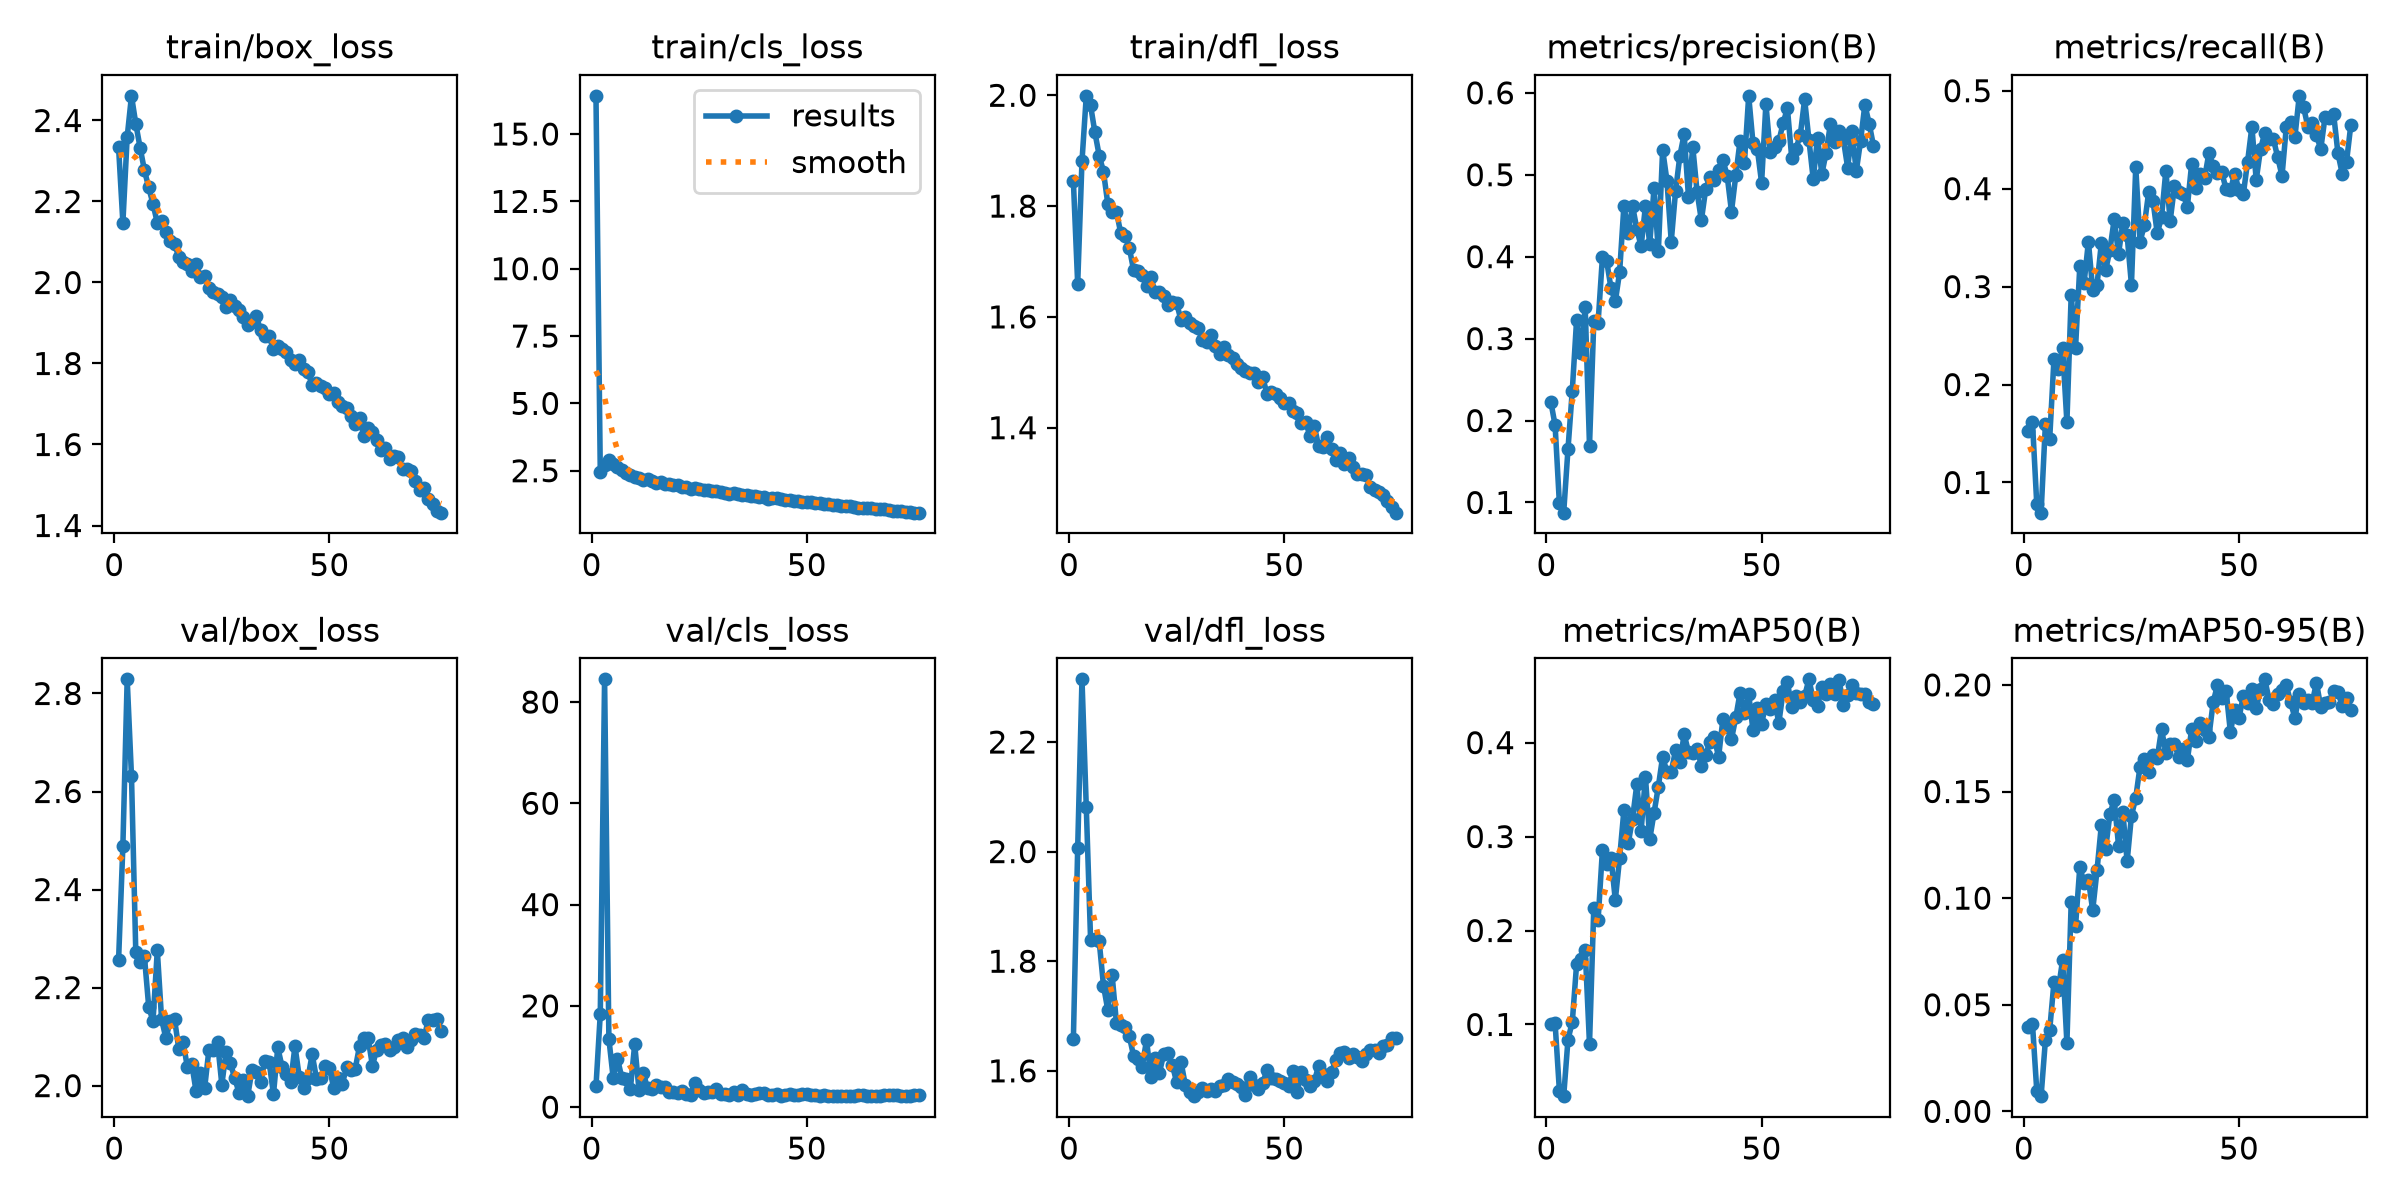
\includegraphics[width=0.72\textwidth]{ch6_train_curves_baseline.png}
\caption{Training losses and training-time validation curves of the baseline (YOLOv8s, RDD2022, 640 px, 76 epochs), as written by the training framework.}
\label{fig:ch6-curves-baseline}
\end{figure}

On the held-out RDD2022 test split (2,784 images, 503 boxes) the baseline reaches mAP\textsubscript{50} 0.497 [0.443, 0.555], mAP\textsubscript{50--95} 0.207 [0.180, 0.239], precision 0.515, recall 0.529, F\textsubscript{1} 0.522 [0.478, 0.562] and 0.090 false positives per image. On HRP4K test it reaches only mAP\textsubscript{50} 0.018, because it never saw HRP4K and the median pothole shrinks to about 10 px at 640 px input. On the manhole probe it reaches mAP\textsubscript{50} 0.368 [0.215, 0.528].

\subsection{Candidate experiment}
The candidate was fine-tuned from the baseline on RDD2022 and HRP4K at 1280 px (Table~\ref{tab:ch5-train}). Its checkpoint was chosen by a rule declared before any test evaluation: the highest mean of RDD2022 and HRP4K validation mAP\textsubscript{50}. The winner, \texttt{epoch25.pt}, led the runner-up by only about 0.0014, so the choice was effectively a tie broken by the rule. Table~\ref{tab:ch6-main} compares the two models at their own thresholds; Figure~\ref{fig:ch6-paired} plots the paired differences.

\begin{table}[!htbp]
\centering
\footnotesize
\renewcommand{\arraystretch}{1.2}
\begin{tabular}{|L{1.5cm}|L{2.4cm}|L{1.9cm}|L{1.9cm}|L{4.6cm}|}
\hline
\textbf{Set} & \textbf{Metric} & \textbf{Baseline, 640 px} & \textbf{Candidate, 1280 px} & \textbf{Difference [95\% CI]} \\
\hline
RDD2022 & mAP\textsubscript{50} & 0.497 & 0.453 & $-$0.0445 [$-$0.0864, $-$0.0059]$^{*}$ \\
\cline{2-5}
test & Precision & 0.515 & 0.454 & $-$0.0608 [$-$0.1055, $-$0.0161]$^{*}$ \\
\cline{2-5}
 & Recall & 0.529 & 0.487 & $-$0.0417 [$-$0.0823, 0.0000] \\
\cline{2-5}
 & FP per image & 0.090 & 0.106 & 0.0158 [0.0004, 0.0314]$^{*}$ \\
\hline
HRP4K & mAP\textsubscript{50} & 0.018 & 0.454 & 0.4354 [0.3915, 0.4792]$^{*}$ \\
\cline{2-5}
test & Recall & 0.019 & 0.416 & 0.3971 [0.3509, 0.4455]$^{*}$ \\
\cline{2-5}
 & FP per image & 0.075 & 0.253 & 0.1776 [0.1304, 0.2278]$^{*}$ \\
\hline
Manhole & mAP\textsubscript{50} & 0.368 & 0.427 & 0.0581 [$-$0.0267, 0.1945] \\
\cline{2-5}
probe & FP per image & 0.222 & 0.291 & 0.0690 [$-$0.0140, 0.1429] \\
\cline{2-5}
 & Manhole hit share & 0.133 & 0.148 & 0.0153 [$-$0.0657, 0.0762] \\
\hline
\end{tabular}
\caption{Results of the baseline and the candidate on the held-out test splits and the manhole probe, each model at the threshold chosen for it on pooled validation data. Each difference is the candidate's value minus the baseline's over paired group-bootstrap resamples, and $^{*}$ marks intervals that do not contain zero. Only the candidate was trained on HRP4K data.}
\label{tab:ch6-main}
\end{table}

\begin{figure}[!htbp]
\centering
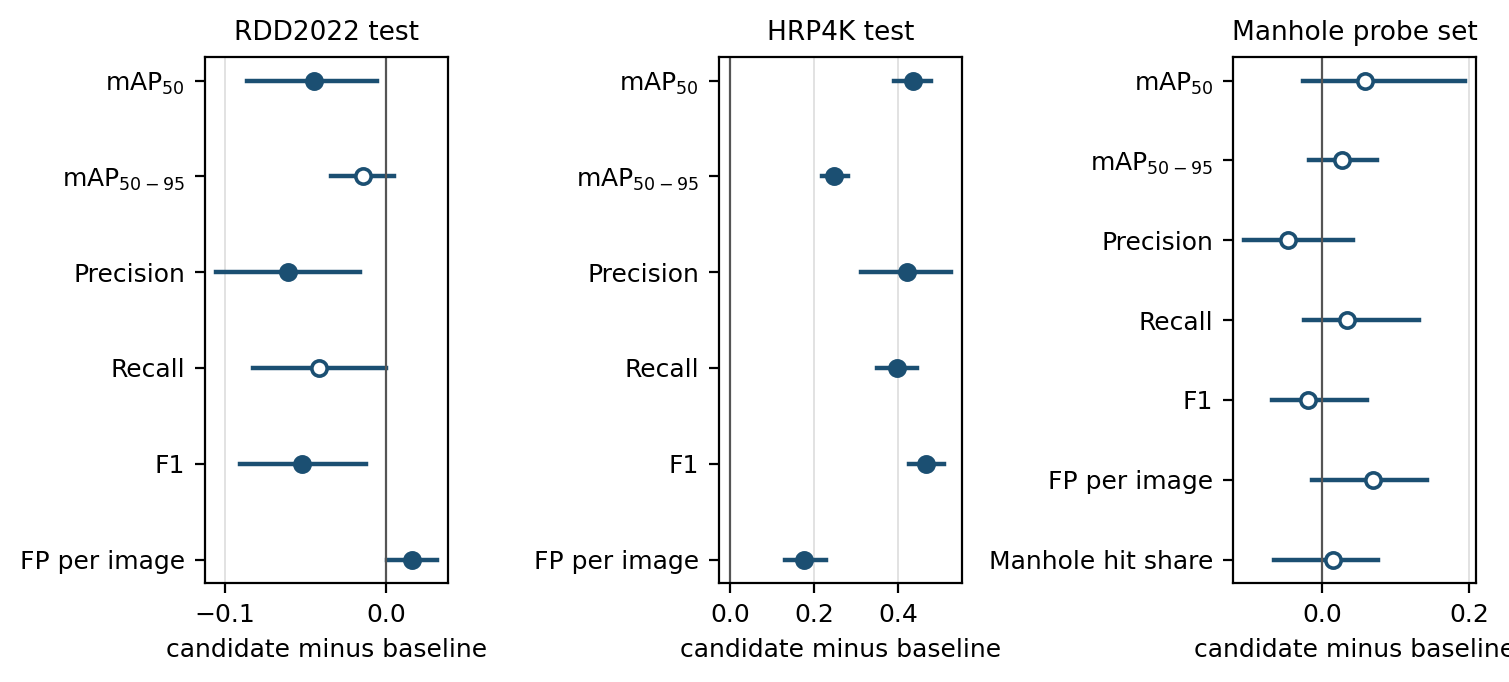
\includegraphics[width=0.95\textwidth]{ch6_paired_differences.png}
\caption{Difference between the candidate and the baseline for each metric, with its 95\% group-bootstrap interval. Filled markers show intervals that do not contain zero, and the panels use different horizontal scales.}
\label{fig:ch6-paired}
\end{figure}

\subsubsection*{Same-resolution checks}
The main comparison mixes data, training and input size. With both models at 640 px, the candidate's RDD2022 test mAP\textsubscript{50} is 0.491 (difference $-$0.0060 [$-$0.0449, 0.0331], not distinguishable), but its precision is lower ($-$0.0898$^{*}$) and it produces more false positives on RDD2022 (+0.0402$^{*}$) and on the probe (0.320 against 0.222 per image$^{*}$); its HRP4K mAP\textsubscript{50} is 0.313 against 0.018. With both at 1280 px, the candidate looks better everywhere, including a lower manhole hit share (0.148 against 0.316), but the baseline is then running at a size it was not trained for, so this is not evidence about the deployed system.

\subsubsection*{Latency}
On the RTX 4060 Laptop GPU (batch 1, forward pass and NMS), the baseline and candidate take 8.16 and 8.19 ms at 640 px in FP32, 17.44 and 16.65 ms at 1280 px in FP32, and 11.02 and 10.62 ms at 1280 px in FP16. Both are YOLOv8s, so cost depends on input size, not on the weights.

\subsection{Interpretation}
The candidate's large gain on HRP4K (mAP\textsubscript{50} 0.018 to 0.454) reflects that it was trained on HRP4K while the baseline never saw it, together with the larger input; it is not a general improvement. At 640 px the candidate still reaches 0.313 on HRP4K, so the gain does not depend on resolution alone, but a single run cannot divide the effect between data and resolution. On RDD2022, which both models were trained on, the candidate is somewhat worse: lower mAP\textsubscript{50}, precision and F\textsubscript{1}, and more false positives per image. We did not demonstrate that the candidate reduces false positives or confusion with manholes compared with the deployed baseline: on the probe the differences have intervals that include zero, and the probe is small (59 pothole boxes, 63 groups). The only comparison favouring the candidate on false positives uses the baseline outside its training resolution. The candidate also differs in data, input size, optimiser and schedule, so one run cannot attribute effects to causes.

\subsection{Validation-only investigations}
Three investigations used validation data only and changed no decision. The candidate's F\textsubscript{1} curve is flat near its peak, staying within 0.01 of the maximum for thresholds from 0.18 to 0.33, and cross-fitting showed that selecting the threshold in-sample is optimistic by only about 0.003 to 0.006 in F\textsubscript{1}. Weighted boxes fusion \cite{solovyev2021wbf} of the baseline at 640 px and the candidate at 960 px gave the same F\textsubscript{1} as the baseline alone on RDD2022 validation (difference 0.001 [$-$0.031, 0.029]) and fell below the candidate on HRP4K validation while costing an extra forward pass, so no ensemble is deployed. Finally, of the candidate's 260 false positives on HRP4K validation, 240 poorly localised or background boxes were categorised in one visual AI pass (Table~\ref{tab:ch6-fp-categories}). Manhole covers account for only 6 (2.5\%), so this analysis does not support manhole confusion as the main error source on HRP4K; 8 boxes appear to lie on unlabelled potholes.

\begin{table}[!htbp]
\centering
\small
\renewcommand{\arraystretch}{1.15}
\begin{tabular}{|l|r|l|r|}
\hline
\textbf{Category} & \textbf{Boxes} & \textbf{Category} & \textbf{Boxes} \\
\hline
Unclear & 101 & Shadow, stain or wet area & 12 \\
\hline
Crack or surface wear & 36 & Plausible unlabelled pothole & 8 \\
\hline
Patch or repair & 32 & Manhole or utility cover & 6 \\
\hline
Road edge or off-road & 27 & Debris or object & 4 \\
\hline
Road marking & 13 & Drain or grate & 1 \\
\hline
\end{tabular}
\caption{Categories of 240 candidate false positives on HRP4K validation images (single AI visual pass; not ground truth).}
\label{tab:ch6-fp-categories}
\end{table}

\subsection{Qualitative comparison on own recordings}
Our 13 recordings from Bengaluru ($1280\times720$, about 30 frames per second, 9,711 frames in total) have no ground truth. Everything in this subsection describes model behaviour and is not a measurement of accuracy, precision, recall or false-positive rate; a higher detection count does not indicate a better model. We ran three models on every frame: the earlier implementation's YOLOv8s-seg model (boxes only, at its own confidence of 0.35, without its stride-5 sampling and ByteTrack tracking), the baseline and the candidate at their validation-selected thresholds. Table~\ref{tab:ch6-totals} gives the totals and Table~\ref{tab:ch6-agreement} the frame-level detection presence.

\begin{table}[!htbp]
\centering
\small
\renewcommand{\arraystretch}{1.15}
\begin{tabular}{|L{4.0cm}|r|r|r|}
\hline
\textbf{Model} & \textbf{Detections} & \textbf{Frames with a detection} & \textbf{Median confidence} \\
\hline
Earlier implementation & 9,665 & 77.29\% & 0.722 \\
\hline
Baseline & 1,913 & 15.91\% & 0.506 \\
\hline
Candidate & 3,049 & 21.73\% & 0.418 \\
\hline
\end{tabular}
\caption{Detections over the 13 recordings (9,711 frames). Behaviour only; no ground truth.}
\label{tab:ch6-totals}
\end{table}

\begin{table}[!htbp]
\centering
\small
\renewcommand{\arraystretch}{1.15}
\begin{tabular}{|L{5.4cm}|r|L{4.6cm}|r|}
\hline
\textbf{Models that fire in the frame} & \textbf{Frames} & \textbf{Models that fire} & \textbf{Frames} \\
\hline
None & 1,537 & Earlier and baseline only & 416 \\
\hline
Earlier implementation only & 5,479 & Earlier and candidate only & 883 \\
\hline
Baseline only & 169 & Baseline and candidate only & 232 \\
\hline
Candidate only & 267 & All three & 728 \\
\hline
\end{tabular}
\caption{Frame-level detection presence of the three models (9,711 frames). These are presence statistics, not accuracy measurements.}
\label{tab:ch6-agreement}
\end{table}

The earlier model fires in most frames, and 3,107 of its 9,665 boxes cover at least 80\% of the frame, which is consistent with the over-segmentation that the Phase 1 report itself recorded on forward-facing footage; neither new model produced such a box. The baseline and the candidate agree on whether a frame contains a detection in 82.13\% of frames. Review strips (Figures~\ref{fig:ch6-strip-pothole} and~\ref{fig:ch6-strip-cover}) were hand-picked to include cases unfavourable to each model and are not representative. In sampled frames both new models also fire on flush manhole covers, patches, stains and paint, so they are not free of look-alike errors, and a visual review of the sampled frames found no clear overall winner between the baseline and the candidate.

\begin{figure}[!htbp]
\centering
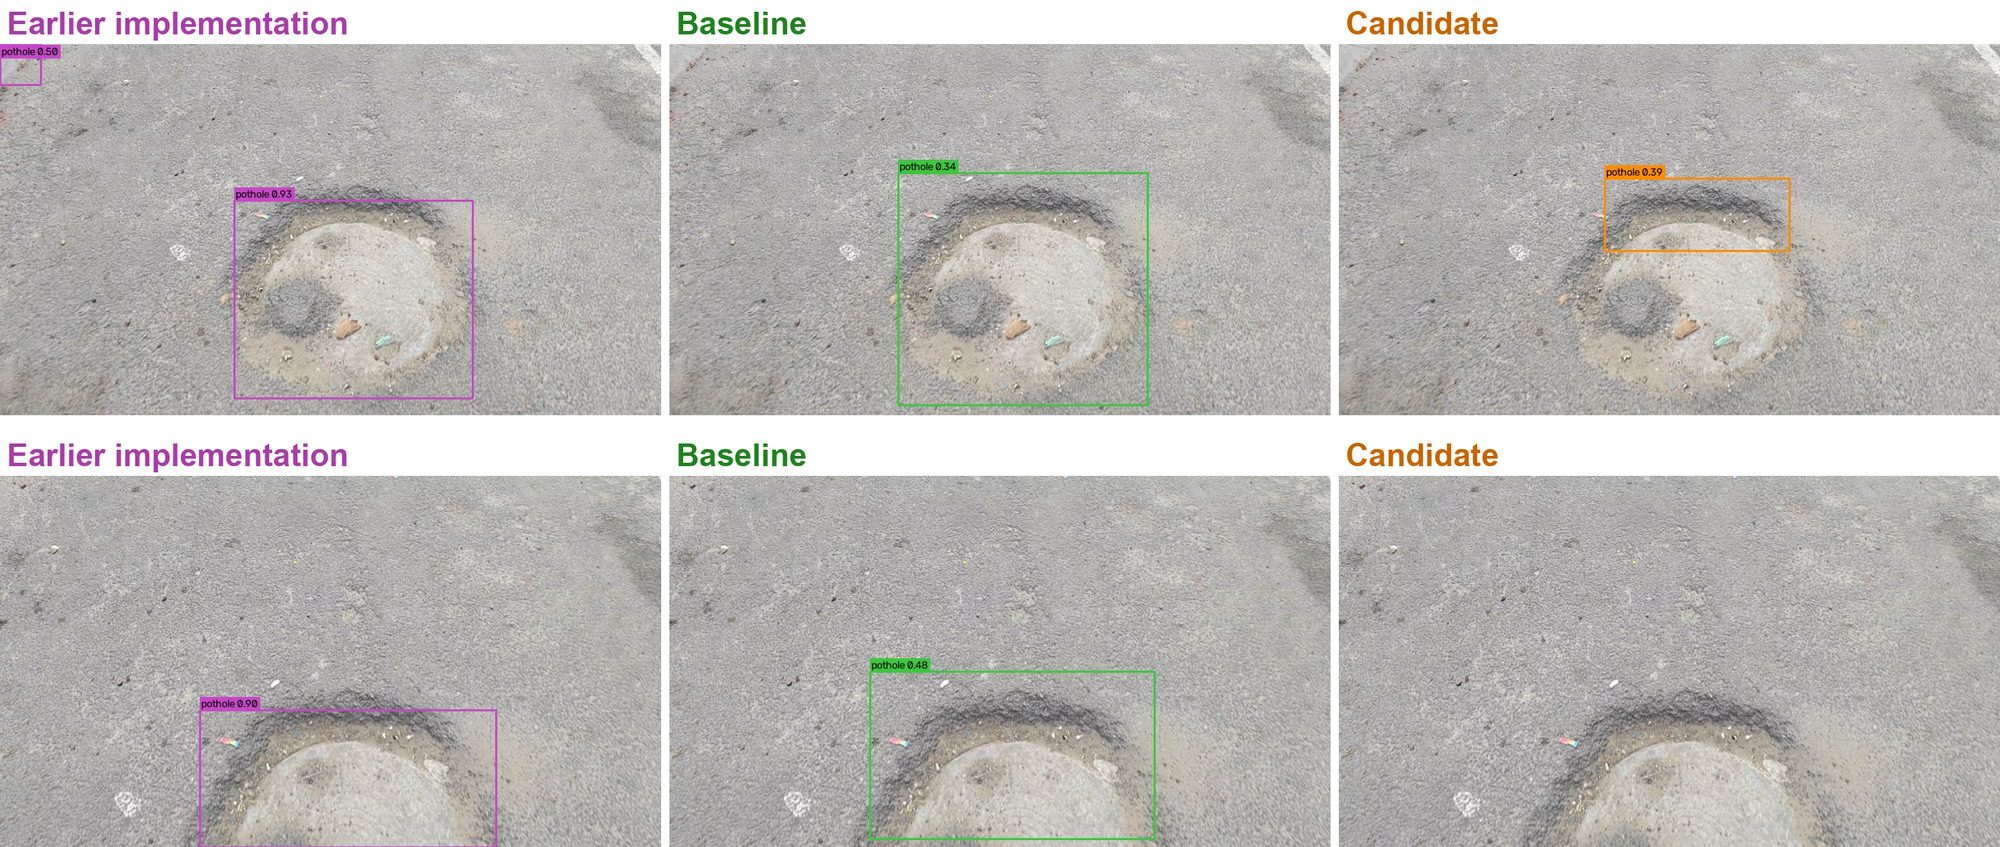
\includegraphics[width=0.82\textwidth]{ch6_strips_round_pothole.jpg}
\caption{Review strip (hand-picked, not representative): a round sunken area of road in two frames of one recording, processed by the earlier implementation, the baseline and the candidate. This is a qualitative view only, since these frames have no ground-truth labels.}
\label{fig:ch6-strip-pothole}
\end{figure}

\begin{figure}[!htbp]
\centering
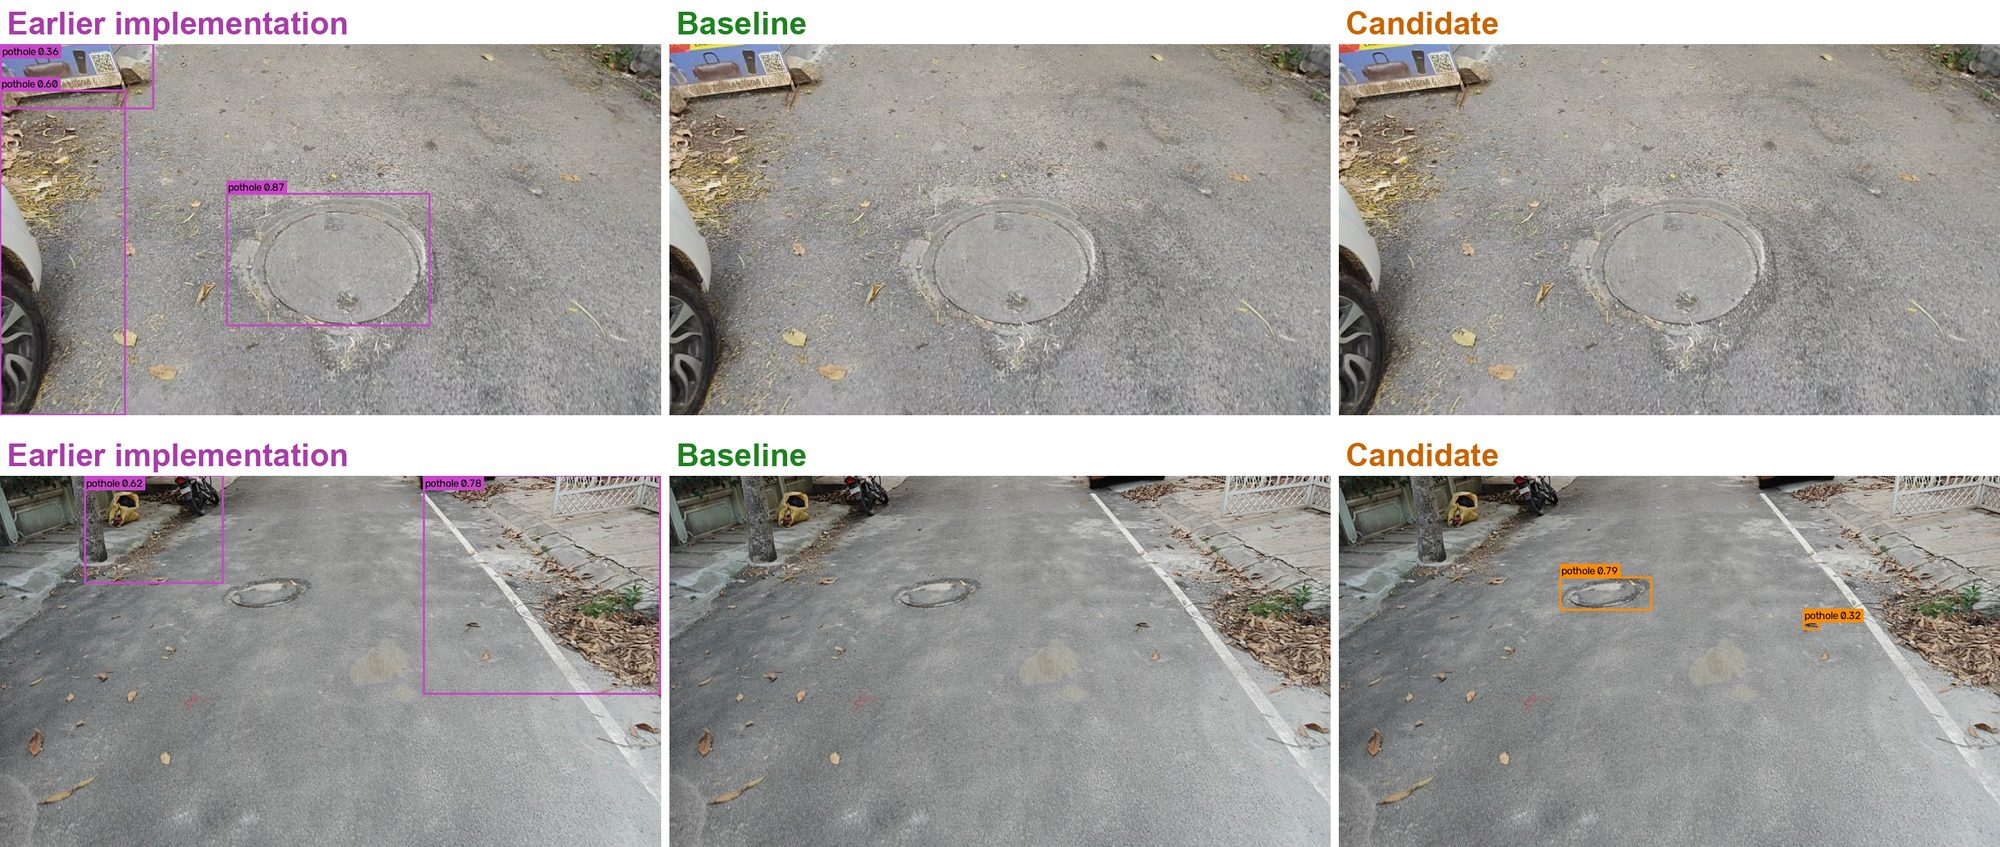
\includegraphics[width=0.82\textwidth]{ch6_strips_manhole_cover.jpg}
\caption{Hand-picked frames, not representative, showing manhole covers set flush with the road in two of our recordings. In the lower frame the candidate draws a box on the cover. These frames have no ground-truth labels, so the comparison is qualitative.}
\label{fig:ch6-strip-cover}
\end{figure}

\subsection{Limitations}
\begin{itemize}[itemsep=0pt]
\item The candidate is one training run with one seed; HRP4K was in-domain for it and was also used to select its epoch and threshold.
\item Label review was a single automated pass that only excluded images; 58\% of HRP4K boxes were judged unclear and kept, and label noise remains.
\item The manhole probe is small (203 images, 63 groups), and all its pothole-free frames contain a manhole by construction.
\item RDD2022 retains scene-level similarity between splits, so its scores are probably optimistic; several country subsets have very few positive test images.
\item No correction for multiple comparisons was applied across the many intervals, and the test splits were evaluated more than once without a log of each run.
\item Our recordings have no ground truth, so no accuracy is known on the roads the system targets.
\item The thresholds of the deployed pipeline, including the 0.25 confidence, the tracking parameters and the 8 m merge radius, are provisional and were never tuned. When we went through 50 confirmed tracks by eye, we judged 8 to be plausible potholes, 11 other road damage, 18 clear false positives and 13 unclear, a subjective count.
\item Route comparison has only been shown on a synthetic session. The system also serves a single user, has no authentication and processes one job at a time.
\end{itemize}

\subsection{Outcome}
We are keeping the baseline as the deployed model. The candidate stays as an experiment, because its only clear gain is on HRP4K, the data it was trained on. On RDD2022 it is somewhat worse, and it did not show fewer false positives or less confusion with manholes. Before the baseline could be replaced, we would need labelled frames from our own roads.

\chapter{Conclusion and Future Work}\label{ch:conclusion}

\section{Conclusion}
We rebuilt the pothole detection and route recommendation system from scratch and evaluated the software and the detector separately. The system takes a road video and a GPS log, detects potholes with a single-class YOLOv8s model, follows each pothole with a motion-aware tracker, merges repeated sightings into mapped potholes, snaps them to an OpenStreetMap road graph and stores the results in SQLite. A FastAPI backend serves a five-tab browser interface and a route planner that runs Dijkstra's algorithm with a cost that adds expected potholes to distance and treats unsurveyed road as unknown. All 1,101 automated tests passed in a full run. The browser interface has no behaviour tests.

For the detector we followed a protocol meant to avoid the mistakes of the earlier implementation. Near-duplicate images were grouped by perceptual hash and kept within one split, label review could only exclude images, thresholds were fixed on validation data before testing, and every comparison carries a group-bootstrap interval. The deployed baseline, YOLOv8s trained on RDD2022 at 640 px, reached mAP\textsubscript{50} 0.497 [0.443, 0.555] on the held-out RDD2022 test split.

The candidate experiment gave a mixed result. Fine-tuned on RDD2022 and HRP4K at 1280 px, the candidate raised HRP4K test mAP\textsubscript{50} from 0.018 to 0.454, a gain explained by training on that data. On RDD2022 its mAP\textsubscript{50} fell by 0.0445 and its false positives per image rose, and it did not demonstrate fewer false positives or less manhole confusion than the baseline. For that reason the deployed model is still the baseline. On our 13 unlabelled recordings the comparison is qualitative: the earlier model produced near-full-frame boxes in 3,107 of its 9,665 detections, and both new models fire on manhole covers, patches and stains.

The implementation also connects to the Sustainable Development Goals set out in Table~\ref{tab:ch1-sdg}. For SDG 9, ordinary road video becomes a pothole map that also records which roads were surveyed. SDG 11 is served by route planning that steers around potholes and states how much evidence supports each route, and SDG 3 by telling drivers about potholes before they reach them. The SDG 11 part has so far been shown only with synthetic data, and none of these effects has been measured in the field.

Some parts of the system are still incomplete. Road condition comes down to a pothole count, a surveyed length and a rate per 100 m for each segment, plus an evidence level for each route, with no severity or grade. Because our recordings cover only about 1,020 m, split across seven stretches that do not connect, route comparison could only be demonstrated on a synthetic session. The system also supports just one user, has no authentication, and still relies on provisional pipeline thresholds.

\section{Future Work}
\begin{enumerate}[itemsep=0pt]
\item Label frames from our own roads, assigning each recording as a whole to a single split. Only then can accuracy be measured on the roads the system is meant for, and only then can we tell whether the baseline or the candidate does better on them.
\item Use a labelled validation set from our roads to choose the confidence, NMS and tracking settings, apply them once to a held-out test set, and log every test evaluation.
\item Train the candidate again with several random seeds, changing the data and the resolution one at a time, to find out what causes its gain on HRP4K and its drop on RDD2022.
\item Turn the stored counts, surveyed lengths and rates into a road-condition score, check it against surveyed road quality, and have the router use it. Estimating severity would need labelled data, which does not exist yet.
\item Record more roads until the surveyed stretches connect at junctions, so that routes can be compared on real data.
\item Before anyone beyond a single local user relies on the system, add authentication, encrypted connections and automated tests for the browser interface.
\end{enumerate}


\clearpage
% ----- References -----
% FIX: one heading only. In the report class, thebibliography prints its own chapter heading
% (\bibname), so the template's extra \chapter*{REFERENCES} is dropped and \bibname is renamed.
% references_generated.tex is written by tools/build_bibliography.py (see README.txt).
\renewcommand{\bibname}{REFERENCES}
% GENERATED by tools/build_bibliography.py from references.bib. Do not edit by hand.
% 54 works, in order of first citation.
\begin{thebibliography}{99}
\addcontentsline{toc}{chapter}{REFERENCES}
\bibitem{morth2023road} Ministry of Road Transport and Highways, Government of India, \textit{{Road Accidents in India 2022}}, Transport Research Wing, Ministry of Road Transport and Highways, New Delhi, 2023. \url{https://pib.gov.in/PressReleasePage.aspx?PRID=1973295}.
\bibitem{redmon2016yolo} J. Redmon, S. Divvala, R. Girshick, and A. Farhadi, ``You only look once: Unified, real-time object detection,'' in \textit{2016 {IEEE} Conference on Computer Vision and Pattern Recognition ({CVPR})}, 2016, pp. 779--788. doi: \url{https://doi.org/10.1109/CVPR.2016.91}.
\bibitem{jocher2023yolov8} G. Jocher, A. Chaurasia, and J. Qiu, \textit{Ultralytics {YOLOv8}}, Software, version 8.0.0, 2023. \url{https://github.com/ultralytics/ultralytics}.
\bibitem{torralba2011unbiased} A. Torralba and A. A. Efros, ``Unbiased look at dataset bias,'' in \textit{CVPR 2011}, 2011, pp. 1521--1528. doi: \url{https://doi.org/10.1109/CVPR.2011.5995347}.
\bibitem{koh2021wilds} P. W. Koh et al., ``{WILDS}: A benchmark of in-the-wild distribution shifts,'' in \textit{Proceedings of the 38th International Conference on Machine Learning}, vol. 139, 2021, pp. 5637--5664. \url{https://proceedings.mlr.press/v139/koh21a.html}.
\bibitem{astm2020d6433} ASTM International, \textit{{Standard Practice for Roads and Parking Lots Pavement Condition Index Surveys}}, Standard D6433-20, 2020. doi: \url{https://doi.org/10.1520/D6433-20}.
\bibitem{eriksson2008pothole} J. Eriksson, L. Girod, B. Hull, R. Newton, S. Madden, and H. Balakrishnan, ``The pothole patrol: using a mobile sensor network for road surface monitoring,'' in \textit{Proceedings of the 6th International Conference on Mobile Systems, Applications, and Services (MobiSys '08)}, 2008, pp. 29--39. doi: \url{https://doi.org/10.1145/1378600.1378605}.
\bibitem{ma2022review} N. Ma et al., ``Computer vision for road imaging and pothole detection: a state-of-the-art review of systems and algorithms,'' \textit{Transportation Safety and Environment}, vol. 4, no. 4, Art. no. tdac026, 2022. doi: \url{https://doi.org/10.1093/tse/tdac026}.
\bibitem{kang2017pothole} B.-H. Kang and S.-I. Choi, ``Pothole detection system using {2D} {LiDAR} and camera,'' in \textit{2017 Ninth International Conference on Ubiquitous and Future Networks (ICUFN)}, 2017, pp. 744--746. doi: \url{https://doi.org/10.1109/ICUFN.2017.7993890}.
\bibitem{kim2022review} Y.-M. Kim, Y.-G. Kim, S.-Y. Son, S.-Y. Lim, B.-Y. Choi, and D.-H. Choi, ``Review of recent automated pothole-detection methods,'' \textit{Applied Sciences}, vol. 12, no. 11, Art. no. 5320, 2022. doi: \url{https://doi.org/10.3390/app12115320}.
\bibitem{maeda2018road} H. Maeda, Y. Sekimoto, T. Seto, T. Kashiyama, and H. Omata, ``Road damage detection and classification using deep neural networks with smartphone images,'' \textit{Computer-Aided Civil and Infrastructure Engineering}, vol. 33, no. 12, pp. 1127--1141, 2018. doi: \url{https://doi.org/10.1111/mice.12387}.
\bibitem{arya2022rdd2022} D. Arya, H. Maeda, S. K. Ghosh, D. Toshniwal, and Y. Sekimoto, ``{RDD2022}: A multi-national image dataset for automatic road damage detection,'' \textit{Geoscience Data Journal}, vol. 11, pp. 846--862, 2024. doi: \url{https://doi.org/10.1002/gdj3.260}.
\bibitem{sahoo2025iwatchroadv2} R. R. Sahoo, S. S. Mohanty, and S. Mishra, \textit{{iWatchRoadv2}: Pothole detection, geospatial mapping, and intelligent road governance}, arXiv preprint arXiv:2510.16375, 2025. \url{https://arxiv.org/abs/2510.16375}.
\bibitem{balakuntala2013pothole} S. Balakuntala and S. Venkatesh, \textit{An intelligent system to detect, avoid and maintain potholes: A graph theoretic approach}, arXiv preprint arXiv:1305.5522, 2013. \url{https://arxiv.org/abs/1305.5522}.
\bibitem{zhang2022bytetrack} Y. Zhang et al., ``{ByteTrack}: Multi-object tracking by associating every detection box,'' in \textit{Computer Vision -- {ECCV} 2022}, 2022, pp. 1--21. doi: \url{https://doi.org/10.1007/978-3-031-20047-2_1}.
\bibitem{luxen2011osrm} D. Luxen and C. Vetter, ``Real-time routing with {OpenStreetMap} data,'' in \textit{Proceedings of the 19th ACM SIGSPATIAL International Conference on Advances in Geographic Information Systems}, 2011, pp. 513--516. doi: \url{https://doi.org/10.1145/2093973.2094062}.
\bibitem{chen2026hrp4k} H. Chen, Z. Tu, Y. Zhao, and J. Ye, ``A high-resolution perspective-view road image dataset for pothole detection,'' \textit{Scientific Data}, vol. 13, no. 1, Art. no. 961, 2026. doi: \url{https://doi.org/10.1038/s41597-026-07317-w}.
\bibitem{safyari2024review} Y. Safyari, M. Mahdianpari, and H. Shiri, ``A review of vision-based pothole detection methods using computer vision and machine learning,'' \textit{Sensors}, vol. 24, no. 17, Art. no. 5652, 2024. doi: \url{https://doi.org/10.3390/s24175652}.
\bibitem{mednis2011real} A. Mednis, G. Strazdins, R. Zviedris, G. Kanonirs, and L. Selavo, ``Real time pothole detection using {Android} smartphones with accelerometers,'' in \textit{2011 International Conference on Distributed Computing in Sensor Systems and Workshops (DCOSS)}, 2011, pp. 1--6. doi: \url{https://doi.org/10.1109/DCOSS.2011.5982206}.
\bibitem{fan2020pothole} R. Fan, U. Ozgunalp, B. Hosking, M. Liu, and I. Pitas, ``Pothole detection based on disparity transformation and road surface modeling,'' \textit{IEEE Transactions on Image Processing}, vol. 29, pp. 897--908, 2020. doi: \url{https://doi.org/10.1109/TIP.2019.2933750}.
\bibitem{dhiman2020pothole} A. Dhiman and R. Klette, ``Pothole detection using computer vision and learning,'' \textit{IEEE Transactions on Intelligent Transportation Systems}, vol. 21, no. 8, pp. 3536--3550, 2020. doi: \url{https://doi.org/10.1109/TITS.2019.2931297}.
\bibitem{ren2017faster} S. Ren, K. He, R. Girshick, and J. Sun, ``Faster {R-CNN}: Towards real-time object detection with region proposal networks,'' \textit{IEEE Transactions on Pattern Analysis and Machine Intelligence}, vol. 39, no. 6, pp. 1137--1149, 2017. doi: \url{https://doi.org/10.1109/TPAMI.2016.2577031}.
\bibitem{zeng2024yolov8pd} J. Zeng and H. Zhong, ``{YOLOv8-PD}: an improved road damage detection algorithm based on {YOLOv8n} model,'' \textit{Scientific Reports}, vol. 14, no. 1, Art. no. 12052, 2024. doi: \url{https://doi.org/10.1038/s41598-024-62933-z}.
\bibitem{arya2021rdd2020} D. Arya, H. Maeda, S. K. Ghosh, D. Toshniwal, and Y. Sekimoto, ``{RDD2020}: An annotated image dataset for automatic road damage detection using deep learning,'' \textit{Data in Brief}, vol. 36, Art. no. 107133, 2021. doi: \url{https://doi.org/10.1016/j.dib.2021.107133}.
\bibitem{arya2020grddc} D. Arya et al., ``Global road damage detection: State-of-the-art solutions,'' in \textit{2020 {IEEE} International Conference on Big Data (Big Data)}, 2020, pp. 5533--5539. doi: \url{https://doi.org/10.1109/BigData50022.2020.9377790}.
\bibitem{arya2021multicountry} D. Arya et al., ``Deep learning-based road damage detection and classification for multiple countries,'' \textit{Automation in Construction}, vol. 132, Art. no. 103935, 2021. doi: \url{https://doi.org/10.1016/j.autcon.2021.103935}.
\bibitem{arya2022crddc} D. Arya et al., ``Crowdsensing-based road damage detection challenge ({CRDDC}'2022),'' in \textit{2022 {IEEE} International Conference on Big Data (Big Data)}, 2022, pp. 6378--6386. doi: \url{https://doi.org/10.1109/BigData55660.2022.10021040}.
\bibitem{chen2026hrp4kzenodo} H. Chen, \textit{{HRP4K}}, Zenodo dataset, version V1.01, 2026. doi: \url{https://doi.org/10.5281/zenodo.21941931}.
\bibitem{giordani2026roaddamage} E. Giordani, L. Arcioni, M. Gil-Mart{\'\i}n, G. L. Foresti, and M. R. Marini, ``Real-world road damage dataset with potholes, cracks, and maintenance holes,'' \textit{Scientific Reports}, vol. 16, no. 1, Art. no. 15318, 2026. doi: \url{https://doi.org/10.1038/s41598-026-46679-4}.
\bibitem{yosinski2014transferable} J. Yosinski, J. Clune, Y. Bengio, and H. Lipson, ``How transferable are features in deep neural networks?'' in \textit{Advances in Neural Information Processing Systems}, vol. 27, 2014, pp. 3320--3328. \url{https://arxiv.org/abs/1411.1792}.
\bibitem{akyon2022sahi} F. C. Akyon, S. O. Altinuc, and A. Temizel, ``Slicing aided hyper inference and fine-tuning for small object detection,'' in \textit{2022 {IEEE} International Conference on Image Processing ({ICIP})}, 2022, pp. 966--970. doi: \url{https://doi.org/10.1109/ICIP46576.2022.9897990}.
\bibitem{barz2020train} B. Barz and J. Denzler, ``Do we train on test data? {Purging CIFAR} of near-duplicates,'' \textit{Journal of Imaging}, vol. 6, no. 6, Art. no. 41, 2020. doi: \url{https://doi.org/10.3390/jimaging6060041}.
\bibitem{kapoor2023leakage} S. Kapoor and A. Narayanan, ``Leakage and the reproducibility crisis in machine-learning-based science,'' \textit{Patterns}, vol. 4, no. 9, Art. no. 100804, 2023. doi: \url{https://doi.org/10.1016/j.patter.2023.100804}.
\bibitem{roberts2017crossvalidation} D. R. Roberts et al., ``Cross-validation strategies for data with temporal, spatial, hierarchical, or phylogenetic structure,'' \textit{Ecography}, vol. 40, no. 8, pp. 913--929, 2017. doi: \url{https://doi.org/10.1111/ecog.02881}.
\bibitem{zauner2011rihamark} C. Zauner, M. Steinebach, and E. Hermann, ``Rihamark: perceptual image hash benchmarking,'' in \textit{Media Watermarking, Security, and Forensics III}, vol. 7880, 2011, p. 78800X. doi: \url{https://doi.org/10.1117/12.876617}.
\bibitem{northcutt2021pervasive} C. G. Northcutt, A. Athalye, and J. Mueller, ``Pervasive label errors in test sets destabilize machine learning benchmarks,'' in \textit{35th Conference on Neural Information Processing Systems (NeurIPS 2021), Track on Datasets and Benchmarks}, 2021. \url{https://arxiv.org/abs/2103.14749}.
\bibitem{padilla2020survey} R. Padilla, S. L. Netto, and E. A. B. da Silva, ``A survey on performance metrics for object-detection algorithms,'' in \textit{2020 International Conference on Systems, Signals and Image Processing (IWSSIP)}, 2020, pp. 237--242. doi: \url{https://doi.org/10.1109/IWSSIP48289.2020.9145130}.
\bibitem{efron1993bootstrap} B. Efron and R. J. Tibshirani, \textit{An Introduction to the Bootstrap}, Springer US, 1993. doi: \url{https://doi.org/10.1007/978-1-4899-4541-9}.
\bibitem{koehn2004significance} P. Koehn, ``Statistical significance tests for machine translation evaluation,'' in \textit{Proceedings of the 2004 Conference on Empirical Methods in Natural Language Processing (EMNLP)}, 2004, pp. 388--395. \url{https://aclanthology.org/W04-3250/}.
\bibitem{bergkirkpatrick2012significance} T. Berg-Kirkpatrick, D. Burkett, and D. Klein, ``An empirical investigation of statistical significance in {NLP},'' in \textit{Proceedings of the 2012 Joint Conference on Empirical Methods in Natural Language Processing and Computational Natural Language Learning}, 2012, pp. 995--1005. \url{https://aclanthology.org/D12-1091/}.
\bibitem{cawley2010overfitting} G. C. Cawley and N. L. C. Talbot, ``On over-fitting in model selection and subsequent selection bias in performance evaluation,'' \textit{Journal of Machine Learning Research}, vol. 11, pp. 2079--2107, 2010. \url{https://jmlr.org/papers/v11/cawley10a.html}.
\bibitem{solovyev2021wbf} R. Solovyev, W. Wang, and T. Gabruseva, ``Weighted boxes fusion: Ensembling boxes from different object detection models,'' \textit{Image and Vision Computing}, vol. 107, Art. no. 104117, 2021. doi: \url{https://doi.org/10.1016/j.imavis.2021.104117}.
\bibitem{haklay2008osm} M. Haklay and P. Weber, ``{OpenStreetMap}: User-generated street maps,'' \textit{IEEE Pervasive Computing}, vol. 7, no. 4, pp. 12--18, 2008. doi: \url{https://doi.org/10.1109/MPRV.2008.80}.
\bibitem{boeing2017osmnx} G. Boeing, ``{OSMnx}: New methods for acquiring, constructing, analyzing, and visualizing complex street networks,'' \textit{Computers, Environment and Urban Systems}, vol. 65, pp. 126--139, 2017. doi: \url{https://doi.org/10.1016/j.compenvurbsys.2017.05.004}.
\bibitem{dijkstra1959note} E. W. Dijkstra, ``A note on two problems in connexion with graphs,'' \textit{Numerische Mathematik}, vol. 1, no. 1, pp. 269--271, 1959. doi: \url{https://doi.org/10.1007/BF01386390}.
\bibitem{paszke2019pytorch} A. Paszke et al., ``{PyTorch}: An imperative style, high-performance deep learning library,'' in \textit{Advances in Neural Information Processing Systems}, vol. 32, 2019. \url{https://papers.nips.cc/paper_files/paper/2019/hash/bdbca288fee7f92f2bfa9f7012727740-Abstract.html}.
\bibitem{wang2020cspnet} C.-Y. Wang, H.-Y. M. Liao, Y.-H. Wu, P.-Y. Chen, J.-W. Hsieh, and I.-H. Yeh, ``{CSPNet}: A new backbone that can enhance learning capability of {CNN},'' in \textit{2020 {IEEE/CVF} Conference on Computer Vision and Pattern Recognition Workshops ({CVPRW})}, 2020, pp. 1571--1580. doi: \url{https://doi.org/10.1109/CVPRW50498.2020.00203}.
\bibitem{lin2017fpn} T.-Y. Lin, P. Doll{\'a}r, R. Girshick, K. He, B. Hariharan, and S. Belongie, ``Feature pyramid networks for object detection,'' in \textit{2017 {IEEE} Conference on Computer Vision and Pattern Recognition ({CVPR})}, 2017, pp. 936--944. doi: \url{https://doi.org/10.1109/CVPR.2017.106}.
\bibitem{liu2018panet} S. Liu, L. Qi, H. Qin, J. Shi, and J. Jia, ``Path aggregation network for instance segmentation,'' in \textit{2018 {IEEE/CVF} Conference on Computer Vision and Pattern Recognition}, 2018, pp. 8759--8768. doi: \url{https://doi.org/10.1109/CVPR.2018.00913}.
\bibitem{li2020generalized} X. Li et al., ``Generalized focal loss: Learning qualified and distributed bounding boxes for dense object detection,'' in \textit{Advances in Neural Information Processing Systems}, vol. 33, 2020, pp. 21002--21012. \url{https://papers.nips.cc/paper/2020/hash/f0bda020d2470f2e74990a07a607ebd9-Abstract.html}.
\bibitem{feng2021tood} C. Feng, Y. Zhong, Y. Gao, M. R. Scott, and W. Huang, ``{TOOD}: Task-aligned one-stage object detection,'' in \textit{2021 {IEEE/CVF} International Conference on Computer Vision ({ICCV})}, 2021, pp. 3490--3499. doi: \url{https://doi.org/10.1109/ICCV48922.2021.00349}.
\bibitem{lin2014coco} T.-Y. Lin et al., ``Microsoft {COCO}: Common objects in context,'' in \textit{Computer Vision -- {ECCV} 2014}, 2014, pp. 740--755. doi: \url{https://doi.org/10.1007/978-3-319-10602-1_48}.
\bibitem{loshchilov2019adamw} I. Loshchilov and F. Hutter, ``Decoupled weight decay regularization,'' in \textit{7th International Conference on Learning Representations (ICLR)}, 2019. \url{https://arxiv.org/abs/1711.05101}.
\bibitem{bochkovskiy2020yolov4} A. Bochkovskiy, C.-Y. Wang, and H.-Y. M. Liao, \textit{{YOLOv4}: Optimal speed and accuracy of object detection}, arXiv preprint arXiv:2004.10934, 2020. \url{https://arxiv.org/abs/2004.10934}.
\end{thebibliography}

\clearpage

% ----- Appendices -----
\appendix
\renewcommand{\thechapter}{\Alph{chapter}}
\renewcommand{\thesection}{\Roman{section}}
% Appendices. Same mechanism as the template: \section titles typed as "Appendix X: ...", Roman section counter.
% This file starts the appendix numbering itself; if main.tex already does the same before \input, the repeats are harmless.
\setcounter{figure}{0}\setcounter{table}{0}
\renewcommand{\thefigure}{A.\arabic{figure}}
\renewcommand{\thetable}{E.\arabic{table}}

\section{Appendix A: Snapshots}
Figure~\ref{fig:appA-water-wet} shows two further review strips from the qualitative comparison on our own recordings (Section~\ref{sec:ch6-results}): a water-filled cavity and a wet patch, each processed by the earlier implementation, the baseline and the candidate, with the confidence of each box drawn on the frame. The frames were picked by hand, include cases unfavourable to each model, and are not representative. There is no ground truth for these recordings.

\begin{figure}[H]
\centering
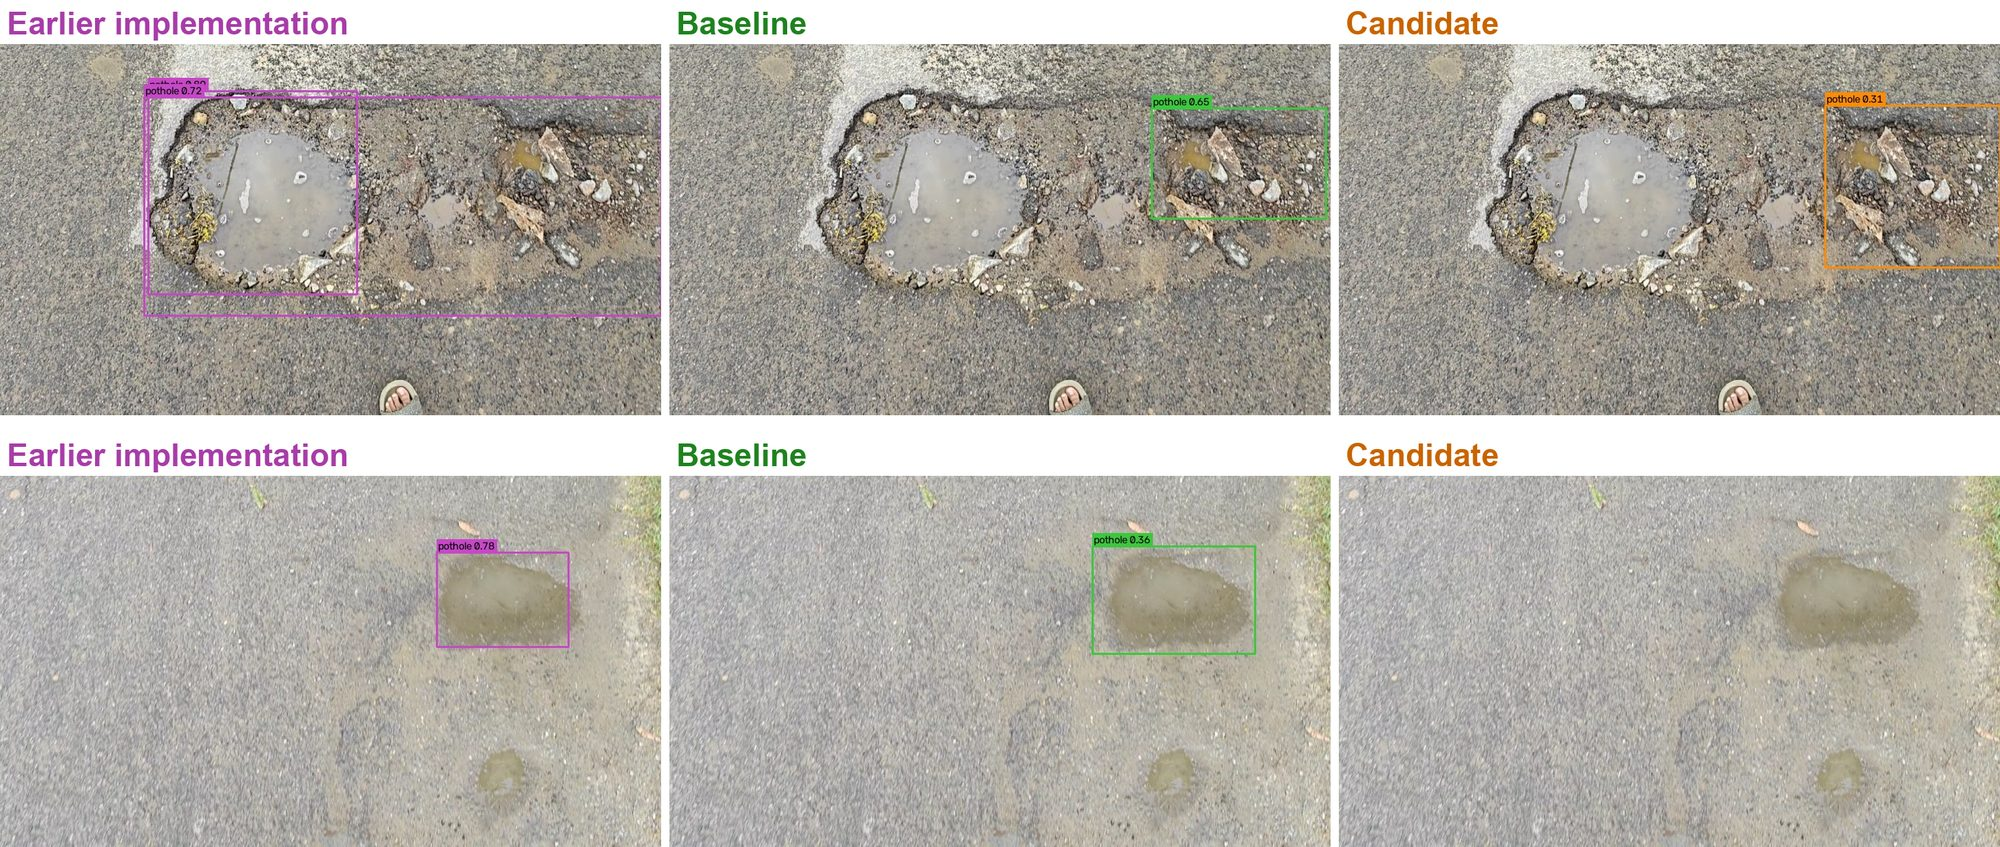
\includegraphics[width=\textwidth]{appA_strips_water_wet.jpg}
\caption{Review strips (hand-picked, not representative): a water-filled cavity (top) and a wet patch (bottom), processed by the earlier implementation, the baseline and the candidate. These frames have no ground-truth labels, so the view is qualitative.}
\label{fig:appA-water-wet}
\end{figure}

% OUTSTANDING: screenshots of the web interface (dashboard, upload, sessions, detections, route planner)
% do not exist yet. Add them here as figures appA_<name>.png when captured.
\clearpage

\section{Appendix B: Details of list of publications related to this project}
\begin{table}[H]
\centering
\renewcommand{\arraystretch}{1.3}
\begin{tabular}{|p{4.6cm}|p{8.6cm}|}
\hline
\textbf{Item} & \textbf{Details} \\
\hline
Author names & Zain Mahedi, Thanu George, Vikas Shashi, Tanish Agrawal (under the guidance of Dr. Seema Patil) \\
\hline
Paper title & AI Powered Pothole Detection and Intelligent Route Optimization System \\
\hline
Name of the conference or journal & 2nd International Conference on Emerging Technologies in Computer Science for Interdisciplinary Applications (Track: Artificial Intelligence and Machine Learning) \\
\hline
Paper ID & 722 \\
\hline
Submission status & Submitted on 30 September 2026 through Microsoft CMT; under review \\
\hline
Place of the conference & To be announced \\
\hline
Date of the conference & To be announced \\
\hline
\end{tabular}
\caption*{Publication submitted by the team. No acceptance has been received.}
\end{table}

The submission describes the earlier phase of this work, the earlier implementation described in Chapter~\ref{ch:intro}, and not the rebuilt system reported here.
\clearpage

\section{Appendix C: Details of Patent}
% No entry. The Phase 1 report left this appendix empty; the team should fill it in or state "Nil".
\clearpage

\section{Appendix D: Details of Funding}
% No entry. The Phase 1 report left this appendix empty; the team should fill it in or state "Nil".
\clearpage

\section{Appendix E: POs and PSOs Mapped}
\setcounter{table}{0}
Each justification below refers to work carried out in the rebuilt system.
% OUTSTANDING: the levels are copied from the Phase 1 report and must be confirmed by the team.

\begin{table}[H]
\centering
\setstretch{1}
\footnotesize
\renewcommand{\arraystretch}{1.1}
\setlength{\tabcolsep}{5pt}
\begin{tabular}{|p{2.7cm}|c|p{8.9cm}|}
\hline
\textbf{PROGRAMME OUTCOMES} & \textbf{Level (1/2/3)} & \textbf{Justification if addressed} \\
\hline
PO1 & 3 & Applies mathematics, statistics, machine learning and geospatial computation: detection metrics and bootstrap intervals, perceptual-hash grouping of images, and a shortest-path route cost on a road graph. \\
\hline
PO2 & 3 & Analyses the shortcomings of the earlier implementation and of the public datasets (leakage between splits, label noise, domain gap) and formulates a single-class box detection problem with a leakage-controlled evaluation. \\
\hline
PO3 & 3 & Designs the complete system: dataset pipeline, detector, tracker, de-duplication of sightings, map matching, route planner, REST API, database and browser interface. \\
\hline
PO4 & 3 & Conducts experiments with group-aware splits, validation-selected thresholds, group-bootstrap intervals and paired comparisons, and reports a negative result for the candidate model. \\
\hline
PO5 & 3 & Uses PyTorch, Ultralytics YOLOv8, OpenCV, FastAPI, SQLite, OSMnx, NetworkX, Leaflet and pytest, and a rented cloud GPU for training. \\
\hline
PO6 & 3 & Addresses road safety by detecting and mapping potholes and by planning routes that account for them; the route comparison is demonstrated on a synthetic session only. \\
\hline
PO7 & 2 & Supports sustainable infrastructure maintenance through data-driven road monitoring from ordinary forward-facing phone or dashcam video and open map data. \\
\hline
PO8 & 2 & Follows ethical practice by using public datasets under their stated licences, flagging licences that were not verified, processing video and location data on the user's own machine, and reporting limitations, the automated review of labels and the negative result openly. \\
\hline
PO9 & 3 & The work was carried out by a team of four under the guidance of the project guide, with the work divided among data preparation, model training and evaluation, application development and testing. \\
\hline
PO10 & 2 & Communicates the work through this report, the project documentation (design decisions, API reference, dataset audit notes) and the browser interface. \\
\hline
PO11 & 2 & Plans the work in phases and keeps cost low through open-source software, public datasets, existing hardware and about \$0.77 of rented GPU time for the candidate training run. \\
\hline
PO12 & 2 & Involves learning new techniques (perceptual hashing, group-bootstrap evaluation, cloud GPU workflow, graph routing) and identifies directions for further work in Chapter~\ref{ch:conclusion}. \\
\hline
\end{tabular}
\caption{Programme Outcomes Mapping with Project}
\end{table}

\begin{table}[H]
\centering
\setstretch{1}
\small
\renewcommand{\arraystretch}{1.3}
\setlength{\tabcolsep}{5pt}
\begin{tabular}{|p{2.7cm}|c|p{8.9cm}|}
\hline
\textbf{PROGRAMME SPECIFIC OUTCOMES} & \textbf{Level (1/2/3)} & \textbf{Justification if addressed} \\
\hline
PSO1 & 2 & Implements a client-server system: a browser client calls a FastAPI REST API with background job processing and SQLite storage on the server. \\
\hline
PSO2 & 3 & Applies software engineering practice (a modular package, validated configuration, 1,101 automated tests, recorded hashes and configurations for reproducible training runs) and machine learning to a real-world problem. \\
\hline
PSO3 & 3 & Integrates computer vision, geospatial data and web technology into one system for road monitoring and route recommendation, demonstrated on recorded video and a synthetic route session. \\
\hline
\end{tabular}
\caption{Programme Specific Outcomes Mapping with Project}
\end{table}
\clearpage

\section{Appendix F: Similarity report, AI Generated report}
\setcounter{figure}{0}\renewcommand{\thefigure}{F.\arabic{figure}}
The report text was checked with Turnitin. Figure~\ref{fig:appF-similarity} shows the similarity summary and Figure~\ref{fig:appF-ai} the AI writing detection summary.

\begin{figure}[H]
\centering
\fbox{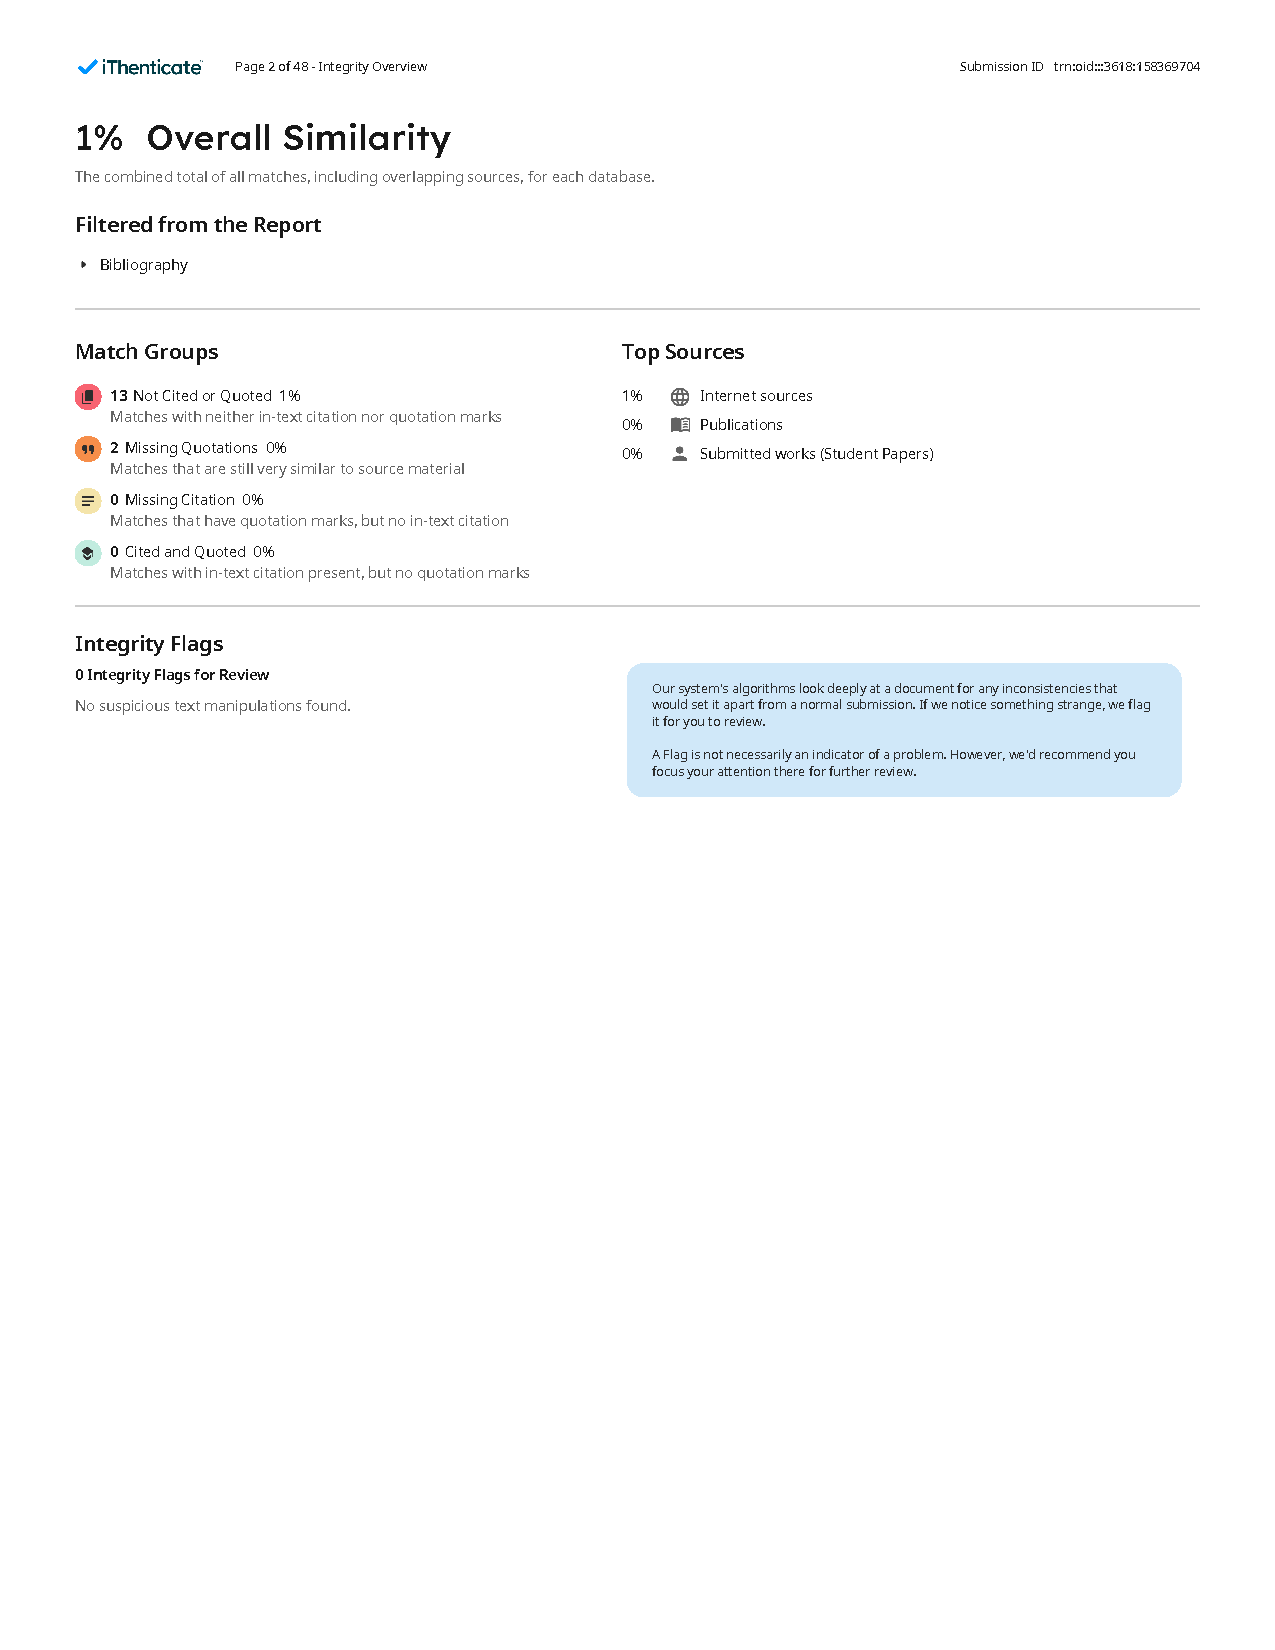
\includegraphics[width=0.97\textwidth]{appF_similarity_report.pdf}}
\caption{Turnitin similarity report summary.}
\label{fig:appF-similarity}
\end{figure}

\begin{figure}[H]
\centering
\fbox{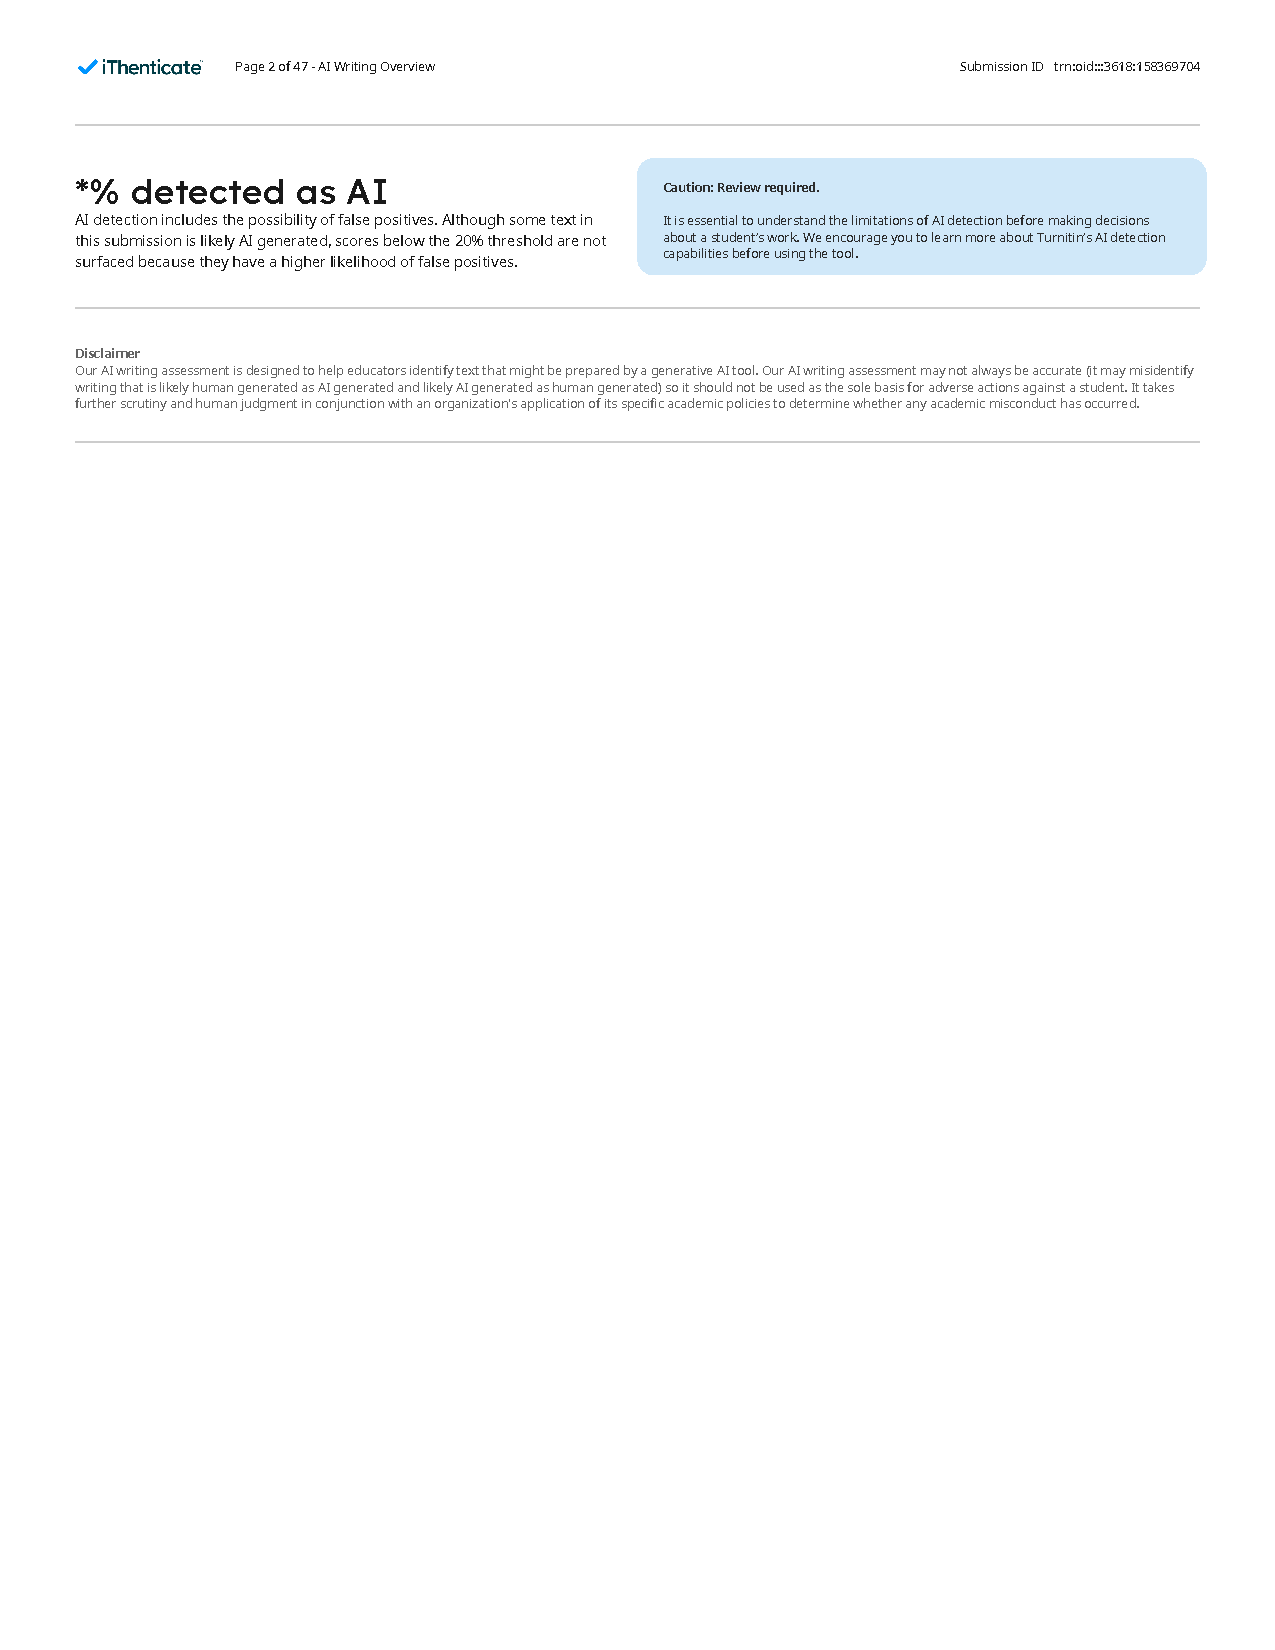
\includegraphics[width=0.97\textwidth]{appF_ai_report.pdf}}
\caption{Turnitin AI writing detection summary.}
\label{fig:appF-ai}
\end{figure}
\clearpage


\end{document}
